\documentclass[a4paper,11pt]{article} 

\usepackage{float}
\usepackage{amsmath}
\usepackage{amssymb}
\usepackage[utf8]{inputenc}
\usepackage{lmodern,textcomp}   
\usepackage[T1]{fontenc}    	
\usepackage{parskip}        	
\usepackage{graphicx}       	
\usepackage{subfigure}
\usepackage{blindtext}
\usepackage{longtable}
\usepackage{epstopdf}       	
\usepackage[english]{babel}	    
\usepackage{hyperref}
\hypersetup{
    colorlinks=true,
    linkcolor=blue,
    filecolor=magenta,      
    urlcolor=cyan,
}
\title{DIY suspension wizard - mountain bike suspension data logger}
\author{Author: Valtteri Turkki}
\date{ \today\ (Original doc: April 4, 2021) }


\begin{document}

\maketitle

\textit{This is a modified version of the original project documentation found at \href{https://wiki.aalto.fi/display/MEX/DIY+suspension+wizard+-+mountain+bike+suspension+data+logger?searchId=LL4XGUSZ1}{wiki.aalto.fi}. It also includes parts from the project plan document that wasn't public, when the project was made.}\\

\vspace{2cm}

\tableofcontents

\newpage
\section{Introduction and motivation}
\rule{12.7cm}{0.4pt}

Mountain bikes have been developed greatly during the last ten years and one of the most aggressively developed bike type has been trail bikes. These are usually full suspension mountain bikes that have suspension travel ranging from 120 to 160 mm and the bikes are designed for going both uphill and downhill easily. This means that the suspension of these bikes is quite complex as it has to be firm under pedalling and still offer blush and controlled ride when going downhill. So, the frame linkage design and also the dampers themselves are quite advanced products. These modern dampers feature a lot of adjustment possibilities without needing to dive into the internal shim stacks. Such adjustments include compression and rebound damping which might even be divided into separate high and low speed adjustments.

So the development has been great, but what about the mere mortal consumer? Despite the great development the consumer still has got the same quantitative indicators about the performance of the suspension, which are O-ring telling how much travel one has used and a stopwatch telling how fast one was. The more sophisticated methods for tuning the suspension are only accessible for world cup riders who have sponsorships with suspension manufacturers.

There have been a few companies that have tried to answer this problem: Motion Instruments and BYB Telemetry offer measurement kits that have all the needed sensors and software, but the prices of these start from 1200 euros. Quartz Shockwiz is a lot cheaper solution at around 300 euros, but it has restrictions as it measures only air pressure. Meaning that coil dampers (that use actual springs) can't be measured and more complex air damper solutions with multiple air chambers are also not measurable with it. So, there is clearly room for DIY solutions in this field.


\newpage
\section{Project plan}
\rule{12.7cm}{0.4pt}

The plan is to create a device that records data from the suspension of a mountain bike and then presents the data in a form that allows the rider to judge whether the adjustments made were good or not. This way the mountain biker should be able to find the correct suspension tune faster, which means that there would be more time for riding the bike. The data recorded from the suspension and the bike will be the linear position of the damper shafts, acceleration of the frame, braking points (brakes on or off) and GPS data. These will be logged to a memory card as a .csv file that is easy to analyze afterwards in Excel or Matlab.  In addition the device might have a wireless connection that allows quick access to the recorded data. Figure \ref{fig:plan_diagram} shows the connections between different components of the device.

\begin{figure}[H]
    \centering
    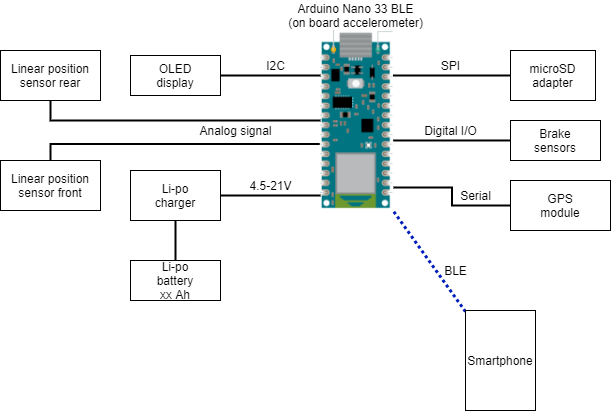
\includegraphics[width=100mm]{Figures/plan_diagram.png}
    \caption{The components of the device and their connections.}
    \label{fig:plan_diagram}
\end{figure}

There were five requirements set for the project and it was split into three stages so that the device was functional after stage 1 and stages 2 and 3 would improve the features of the device. The five requirements are:

\begin{enumerate}
\item The measurements have to be reasonably accurate and the acquired data should be meaningful in a way that it can be used for suspension tuning and generally experimenting with suspension characteristics.

\item The device must be suitable for mountain bike use, meaning that it will need to be portable, small and it should withstand the elements.

\item The device is as universal as reasonably possible, meaning that it really measures the suspension travel, not air chamber pressure or something else, and can fit most bikes. One aspect is also that the device should be easily improvable in the future e.g. the whole thing doesn't need to be re-engineered if one wants to for instance put a Raspberry pi zero inside instead of Arduino Nano.

\item Overview of the data should be accessible without connecting the device to PC.

\item (Bonus) The project should be so cheap and functional that it would really become appealing for the average rider to build this by oneself.
\end{enumerate}

The three stages are following: Stage one is to fulfill the first three requirements i.e., have a working device that produces a bunch of numbers. Second stage is to improve the usability of the device for instance with better user-interface and with more advanced features, such as automatic recording based on gpx-file track segments. The third stage is to implement a phone app that allows the user to see an overview of the recorded data on the fly without a laptop. The bonus goal about the cost will be estimated in the end and the final report might have alternative parts lists so that one can choose the suitable cost and feature level, if one decides to build this.


\newpage
\section{Components for the project}
\rule{12.7cm}{0.4pt}

As the device needs to be small and portable, the components were selected so that the are power efficient and fit in a small enclosure. The component list is shown in table \ref{tab:components} below.

\begin{table}[H]
    \caption{The components used for the project along with their prices and quantities.}
    \centering
    \begin{tabular}{ |p{0.2\linewidth} | p{0.3\linewidth}| p{0.07\linewidth}| p{0.1\linewidth}| p{0.2\linewidth}| } 
     \hline
     Component & Model & Qty & Price & Sourced from \\ 
     \hline
     \hline
     Microcontroller &	Arduino Nano 33 BLE &	1 &	31.16€ &	Elfa Distrelec\\
     \hline
     GPS module &	Arduino mkr GPS shield &	1 &	32.56€ &	Elfa Distrelec\\
     \hline
     MicroSD adapter &	Adafruit 254 &	1 &	9.85€ &	Elfa Distrelec\\
     \hline
     LiPo charger &	Adafruit 1944 &	1 &	18.40€ &	Elfa Distrelec\\
     \hline
     Battery &	1350 mAh 3.7 V LiPo battery &	1 &	14.50€ &	Partco\\
     \hline
     OLED display &	32x128 I2C display with SSD1306 driver &	1 &	9.90€ &	Own storage\\
     \hline
     Potentiometers &	Vishay 20 kohm 10 turn, 534B1203JBC &	2 &	14.40€ &	Partco\\
     \hline
     Micro switches &	Omron NC ip67 miniature switch &	2 &	1.08€ &	Elfa Distrelec\\
     \hline
     Sensor connectors &	SP13 ip68 connectors (4 and 5 pole models) &	2+2	& 5.95€ &	Partco\\
     \hline
     Push buttons &	Ip67 NO push button 0.4 A 32 V &	2 &	$\approx$10€ &	Own storage\\
     \hline
     Electric components & Active buzzer, 2x diodes, 2x resistor(1K and 3K), ON-OFF switch, DC21 jack and wires & - & $\approx$5€ &	Own storage\\
     \hline
     Mechanical parts & Bunch of M3 nuts and bolts, 2x spiral springs, piece of Plexiglass and some O-rings & - & - & Own storage / springs from old key chains\\
     \hline
     3D printer filament &	Prusament PETG 1.75 mm orange 1 kg spool &	1 &	29.99€ &	Prusa research a.s.\\
     \hline
    \end{tabular}
    \label{tab:components}
\end{table}

The microcontroller unit for the project was chosen to be Arduino nano 33 BLE. The reasons for choosing that board are that it features integrated Bluetooth and IMU, so it helps to keep the size down. It also features 12-bit analog to digital converter and more processor power and memory than a standard nano. These might come handy as a bit similar project in 2017 mentioned that uno didn't provide enough computing power for reasonable sampling rates. An interesting feature of the nano 33 BLE is also that it can use Mbed RTOS features. The Arduino GPS module was chosen because it was quite cheap and the idea was that the Arduino library should work flawlessly with the Nano (though it didn't). The filament was chosen to be PETG (polyethylene terephthalate modifed with glycol) rather than PLA (polylactic acid) since PETG is a bit more flexible, so if the print bends it won't crack immediately. All 3D printing for the project was done with Prusa Mini FDM printer and slicing was done with PrusaSlicer software. The 3D models were made using Solidworks CAD software.



\newpage
\section{Project progress}
\rule{12.7cm}{0.4pt}

The project began with ordering the components and designing the mechanical parts. The components arrived on the second week of February and as they arrived they were tested to work individually. This already brought the first problems as the Arduino\_MKRGPS library is not compatible with the Mbed architecture of the Nano 33 BLE, so after trying different libraries the TinyGPS++ library by Mikal Hart proved to be working quite well. Second library problem was found when testing the on board IMU, as it has range of ±16g, but the Arduino\_LSM9DS1 library does not allow you to change that from the default range of ±4g. Fortunately there was a version 2.0 from that library in github written by Femme Verbeek. This version not only allowed changing the measuring range, but also calibrating, filtering and changing the sample rate of the IMU.

Now when the library issues were tackled, the work focused on the mechanical parts. These include the sensor design for the potentiometers and micro switches and designing a compact enclosure for the electronics. The key sensors of this device are the linear position sensors that measure the suspension travel. A weatherproof linear potentiometer would have been the best choice, but those are so expensive that they weren't really an option. Instead, the sensors were made using a multi-turn potentiometer combined with a spiral spring and string. These were used to make a DIY string potentiometer that works basically like an electric ruler. After a couple of iterations the most frictionless design was obtained and the finalized versions were printed and assembled. Figure \ref{fig:string_pots} (a) shows the linear sensor internal design and figure \ref{fig:string_pots} (b) shows the sensor mounted to a suspension fork.

\begin{figure}[H]
    \hfill
    \subfigure[]{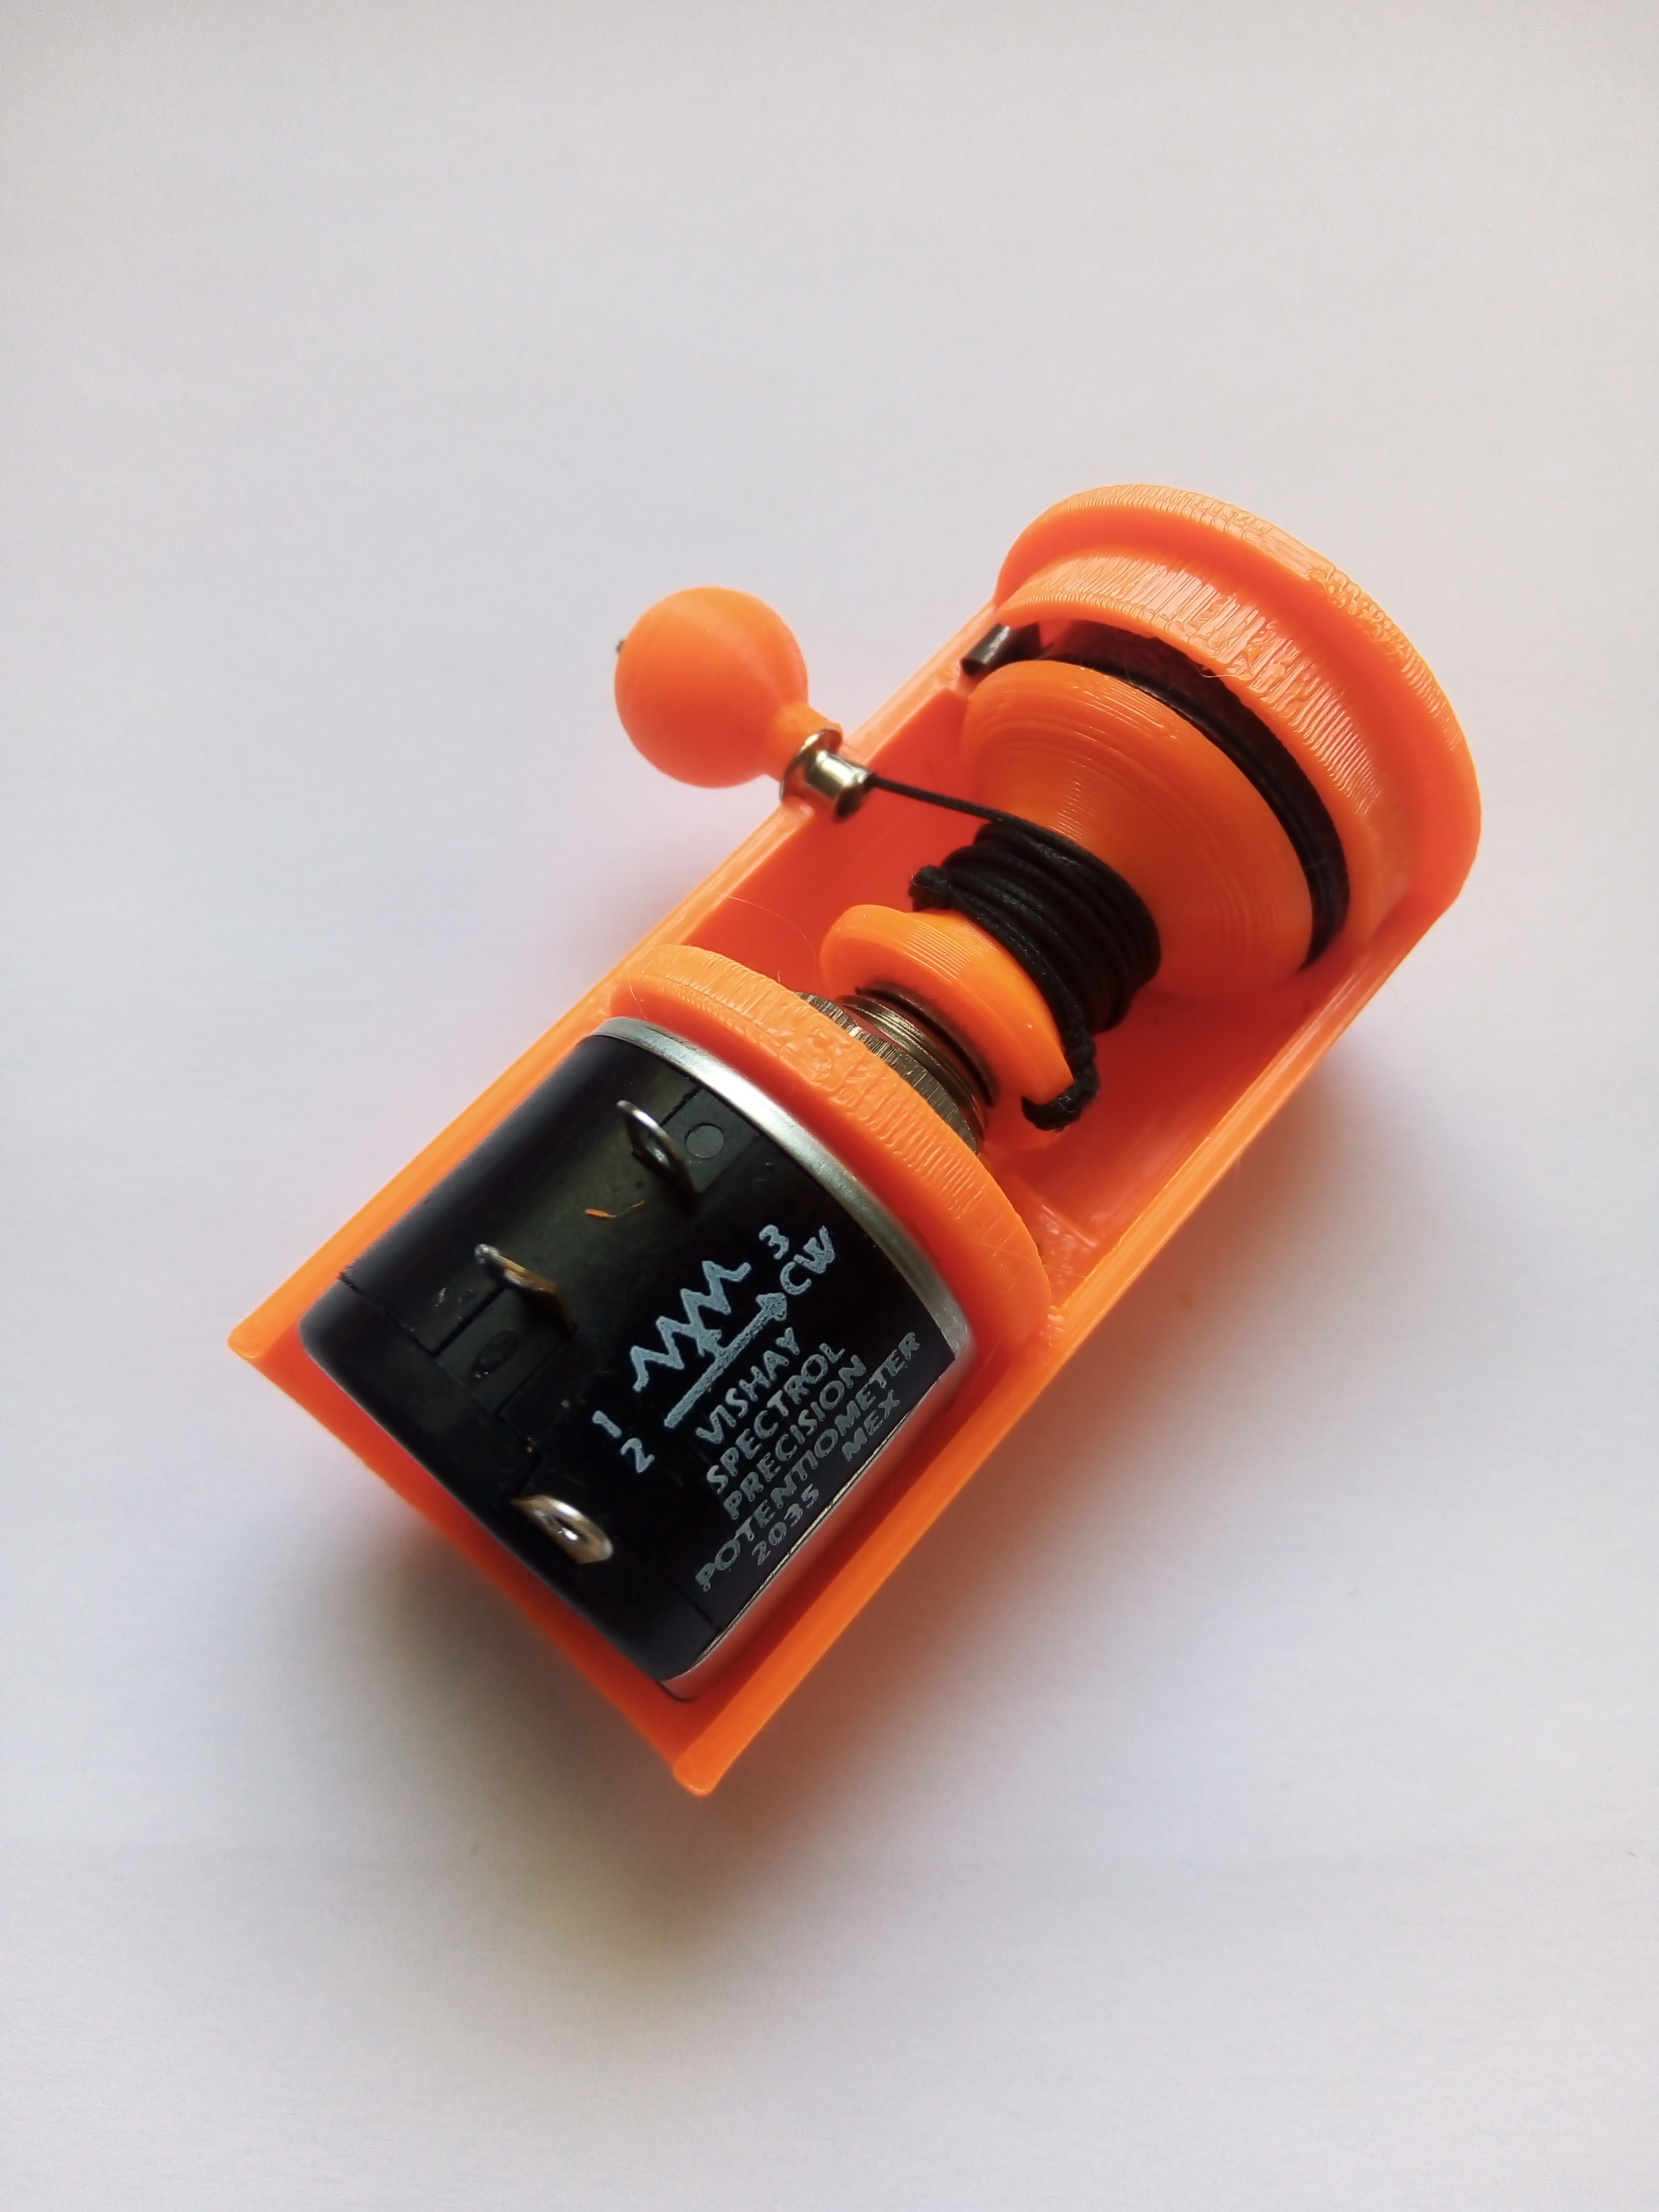
\includegraphics[height=10cm]{Figures/sensor_v2_2.jpg}}
    \hfill
    \subfigure[]{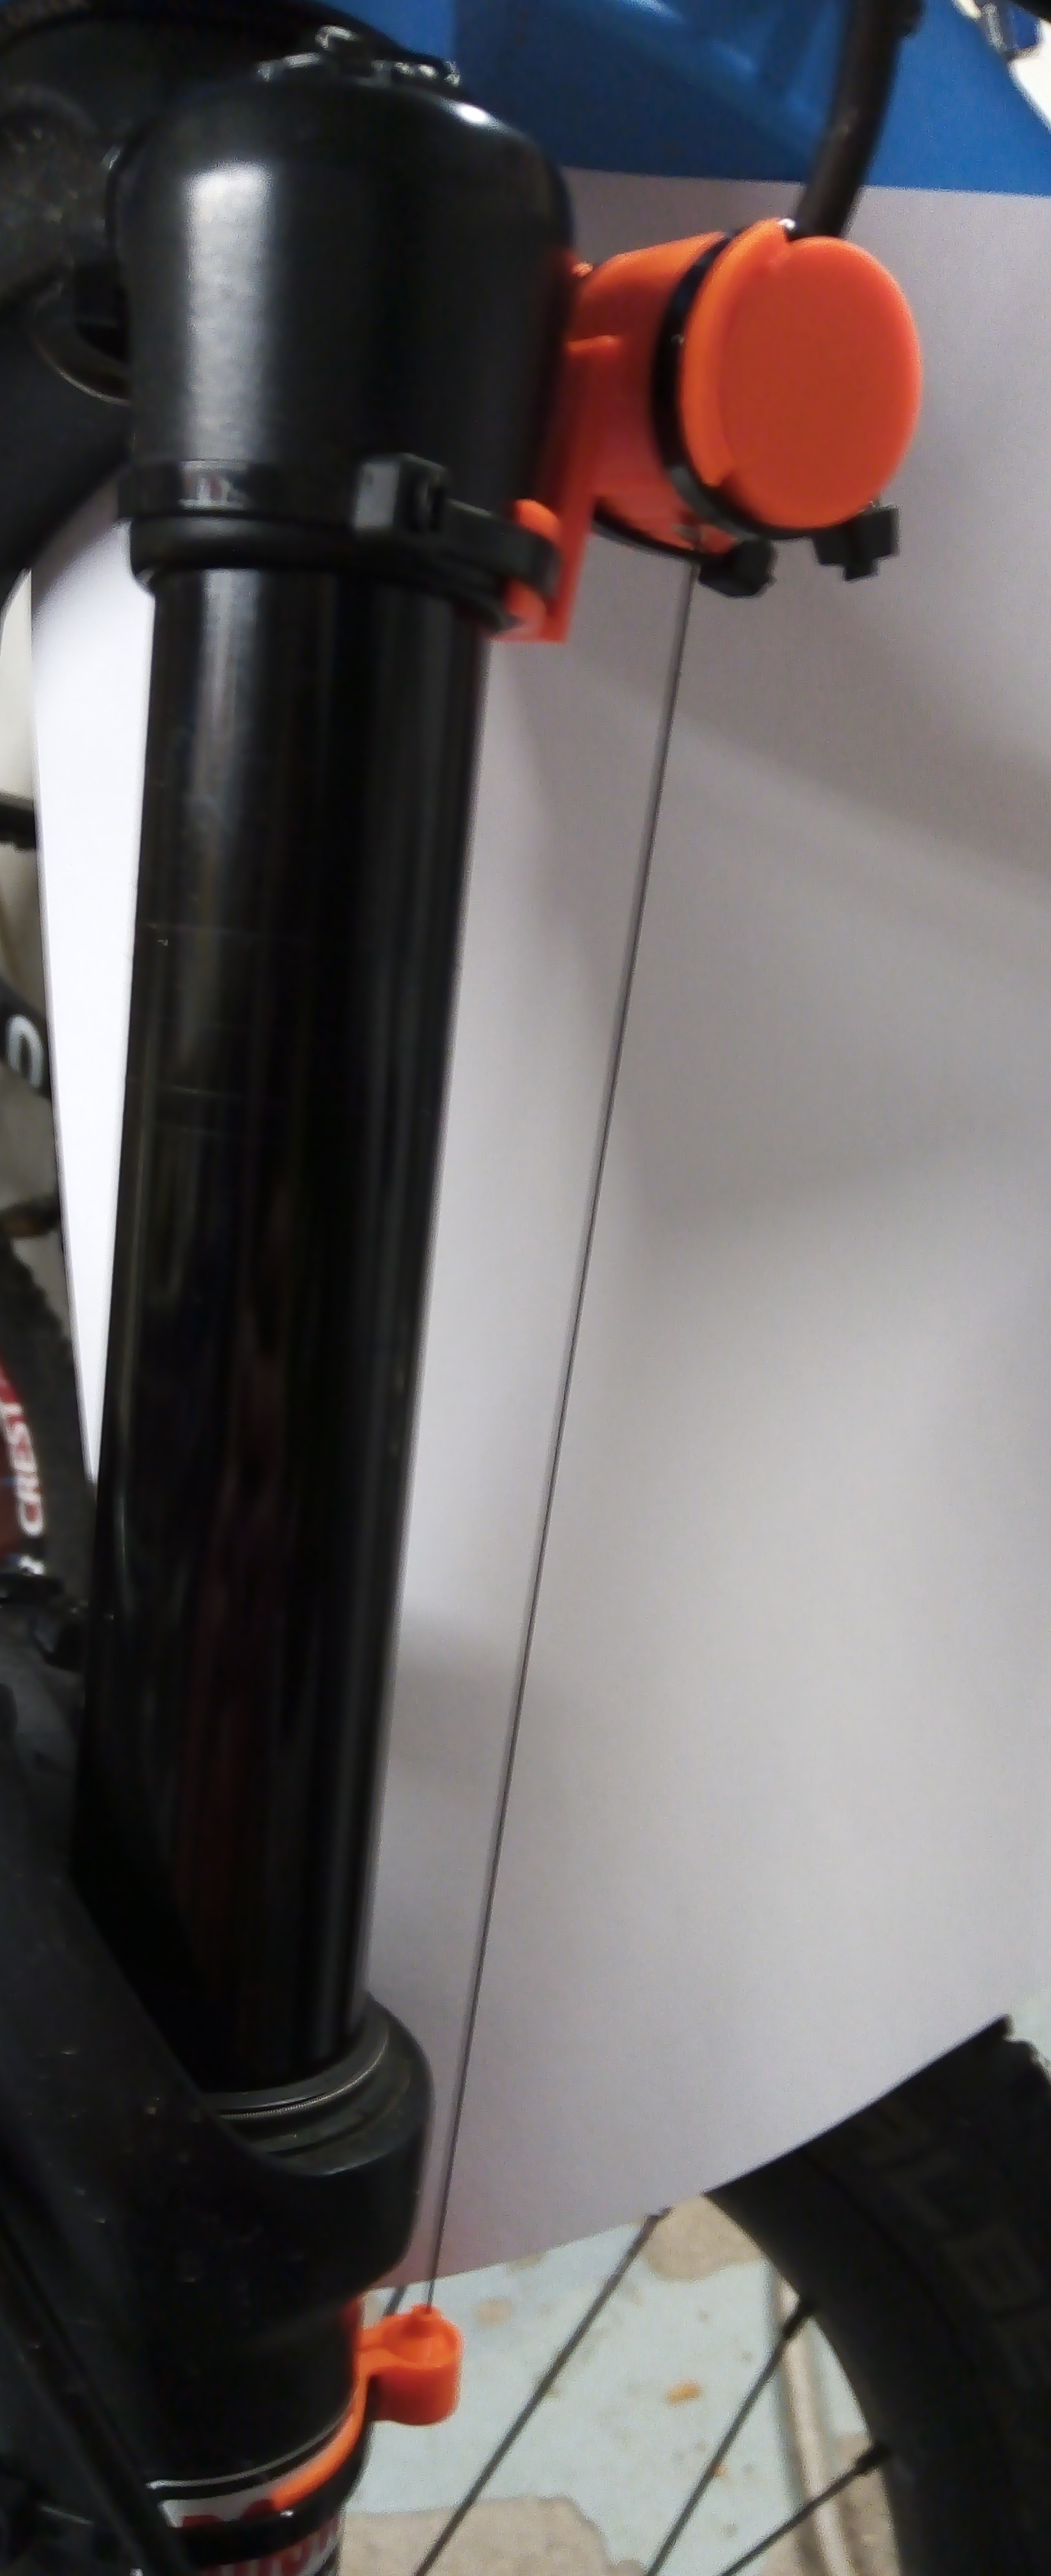
\includegraphics[height=10cm]{Figures/pot_assembled.jpg}}
    \hfill
    \caption{(a) The internal design of the string potentiometer: The spiral spring is in the far end, while the 10-turn potentiometer is in the front. (b) The string pot assembled to a suspension fork using the 3D printed mounts and zip ties.}
    \label{fig:string_pots}
\end{figure}

The diameter of the reel is 8 mm, which gives the sensor an overall range of around 250 mm. This should be enough for all suspension forks and more than enough for rear shocks. The ball at the end of the string is meant to work as a safety feature: If the string gets caught on a branch or stick when riding, the ball joint should  break free and prevent the sensor from breaking. The ball joint also makes it easy to mount the sensor on to different shape and size damper bodies as only a 3D printed adapter needs to be used.

The brake sensor was a lot simpler to design than the potentiometer as it is only an on-off sensor. It was designed so that the lever of the micro switch is inserted against the brake lever so that it contacts the reach adjusting bolt in front of the lever body and when the rider pulls the lever the switch opens. Because the sensor is attached using cable ties, the position can be adjusted so that the sensor reading matches the bite point of the brakes. The micro switch was printed in place so that the sensor is watertight without any further sealing. Figure \ref{fig:brake_sensor} below shows the brake sensor attached on to its place.

\begin{figure}[H]
    \centering
    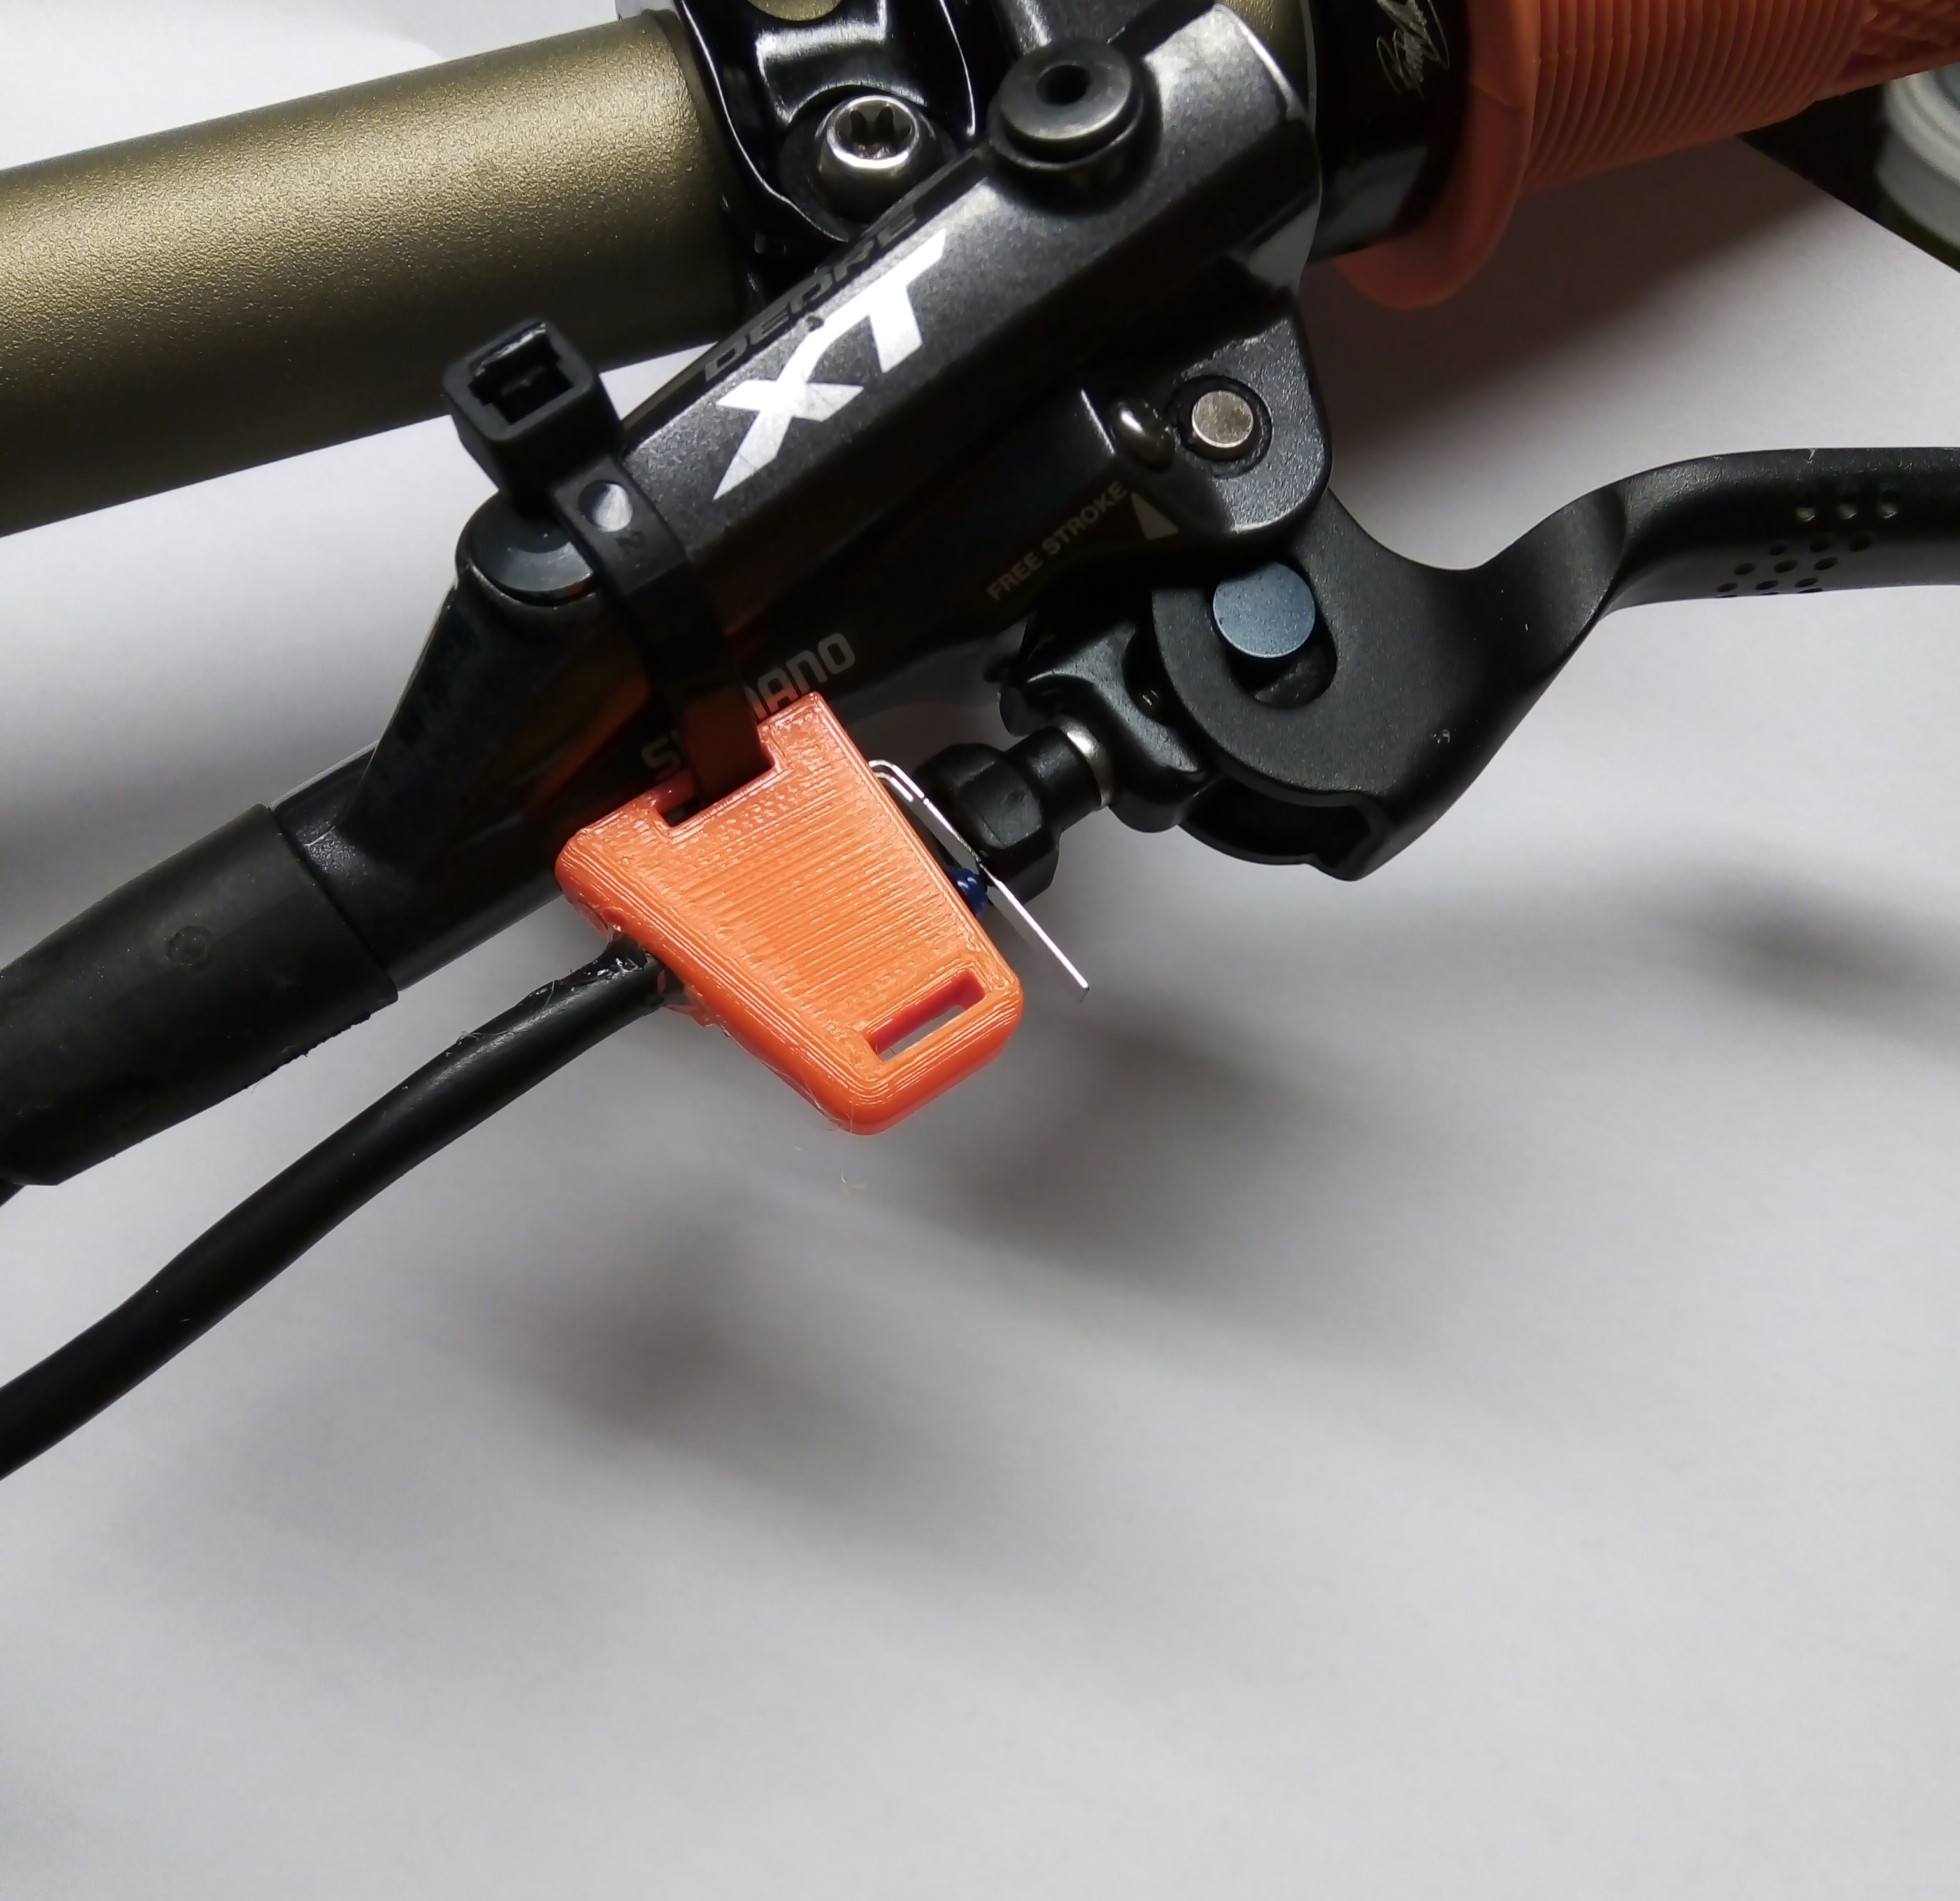
\includegraphics[width=80mm]{Figures/brake_sensor_1.jpg}
    \caption{The brake sensor that utilizes a micro switch installed to a brake lever using a zip tie. The braking event is determined from the movement of the reach adjuster knob, which presses the lever of the switch and closes it, when the brake lever is not being pulled.}
    \label{fig:brake_sensor}
\end{figure}

The only possible issue with the design in figure \ref{fig:brake_sensor} is that, if the lever is straight and doesn't have a reach adjusting bolt, it might be hard to find contact point for the micro switch lever. Fortunately all modern hydraulic mountain bike disc brake levers tend to have a reach adjusting bolt so this issue is quite unlikely to occur.

Now as the external sensors were designed it was time to focus to the electronics side and after that design the enclosure for those. Plan was to test the device on breadboard before soldering everything together. This failed though, because there were so many jumper wires that the used breadboard leads didn't make contact to all of them. This meant that the circuit plan was checked once more and then it was time to solder. The decorated pcb is shown in figure \ref{fig:pcb_plain} (a) \& (b) below.

\begin{figure}[H]
    \hfill
    \subfigure[]{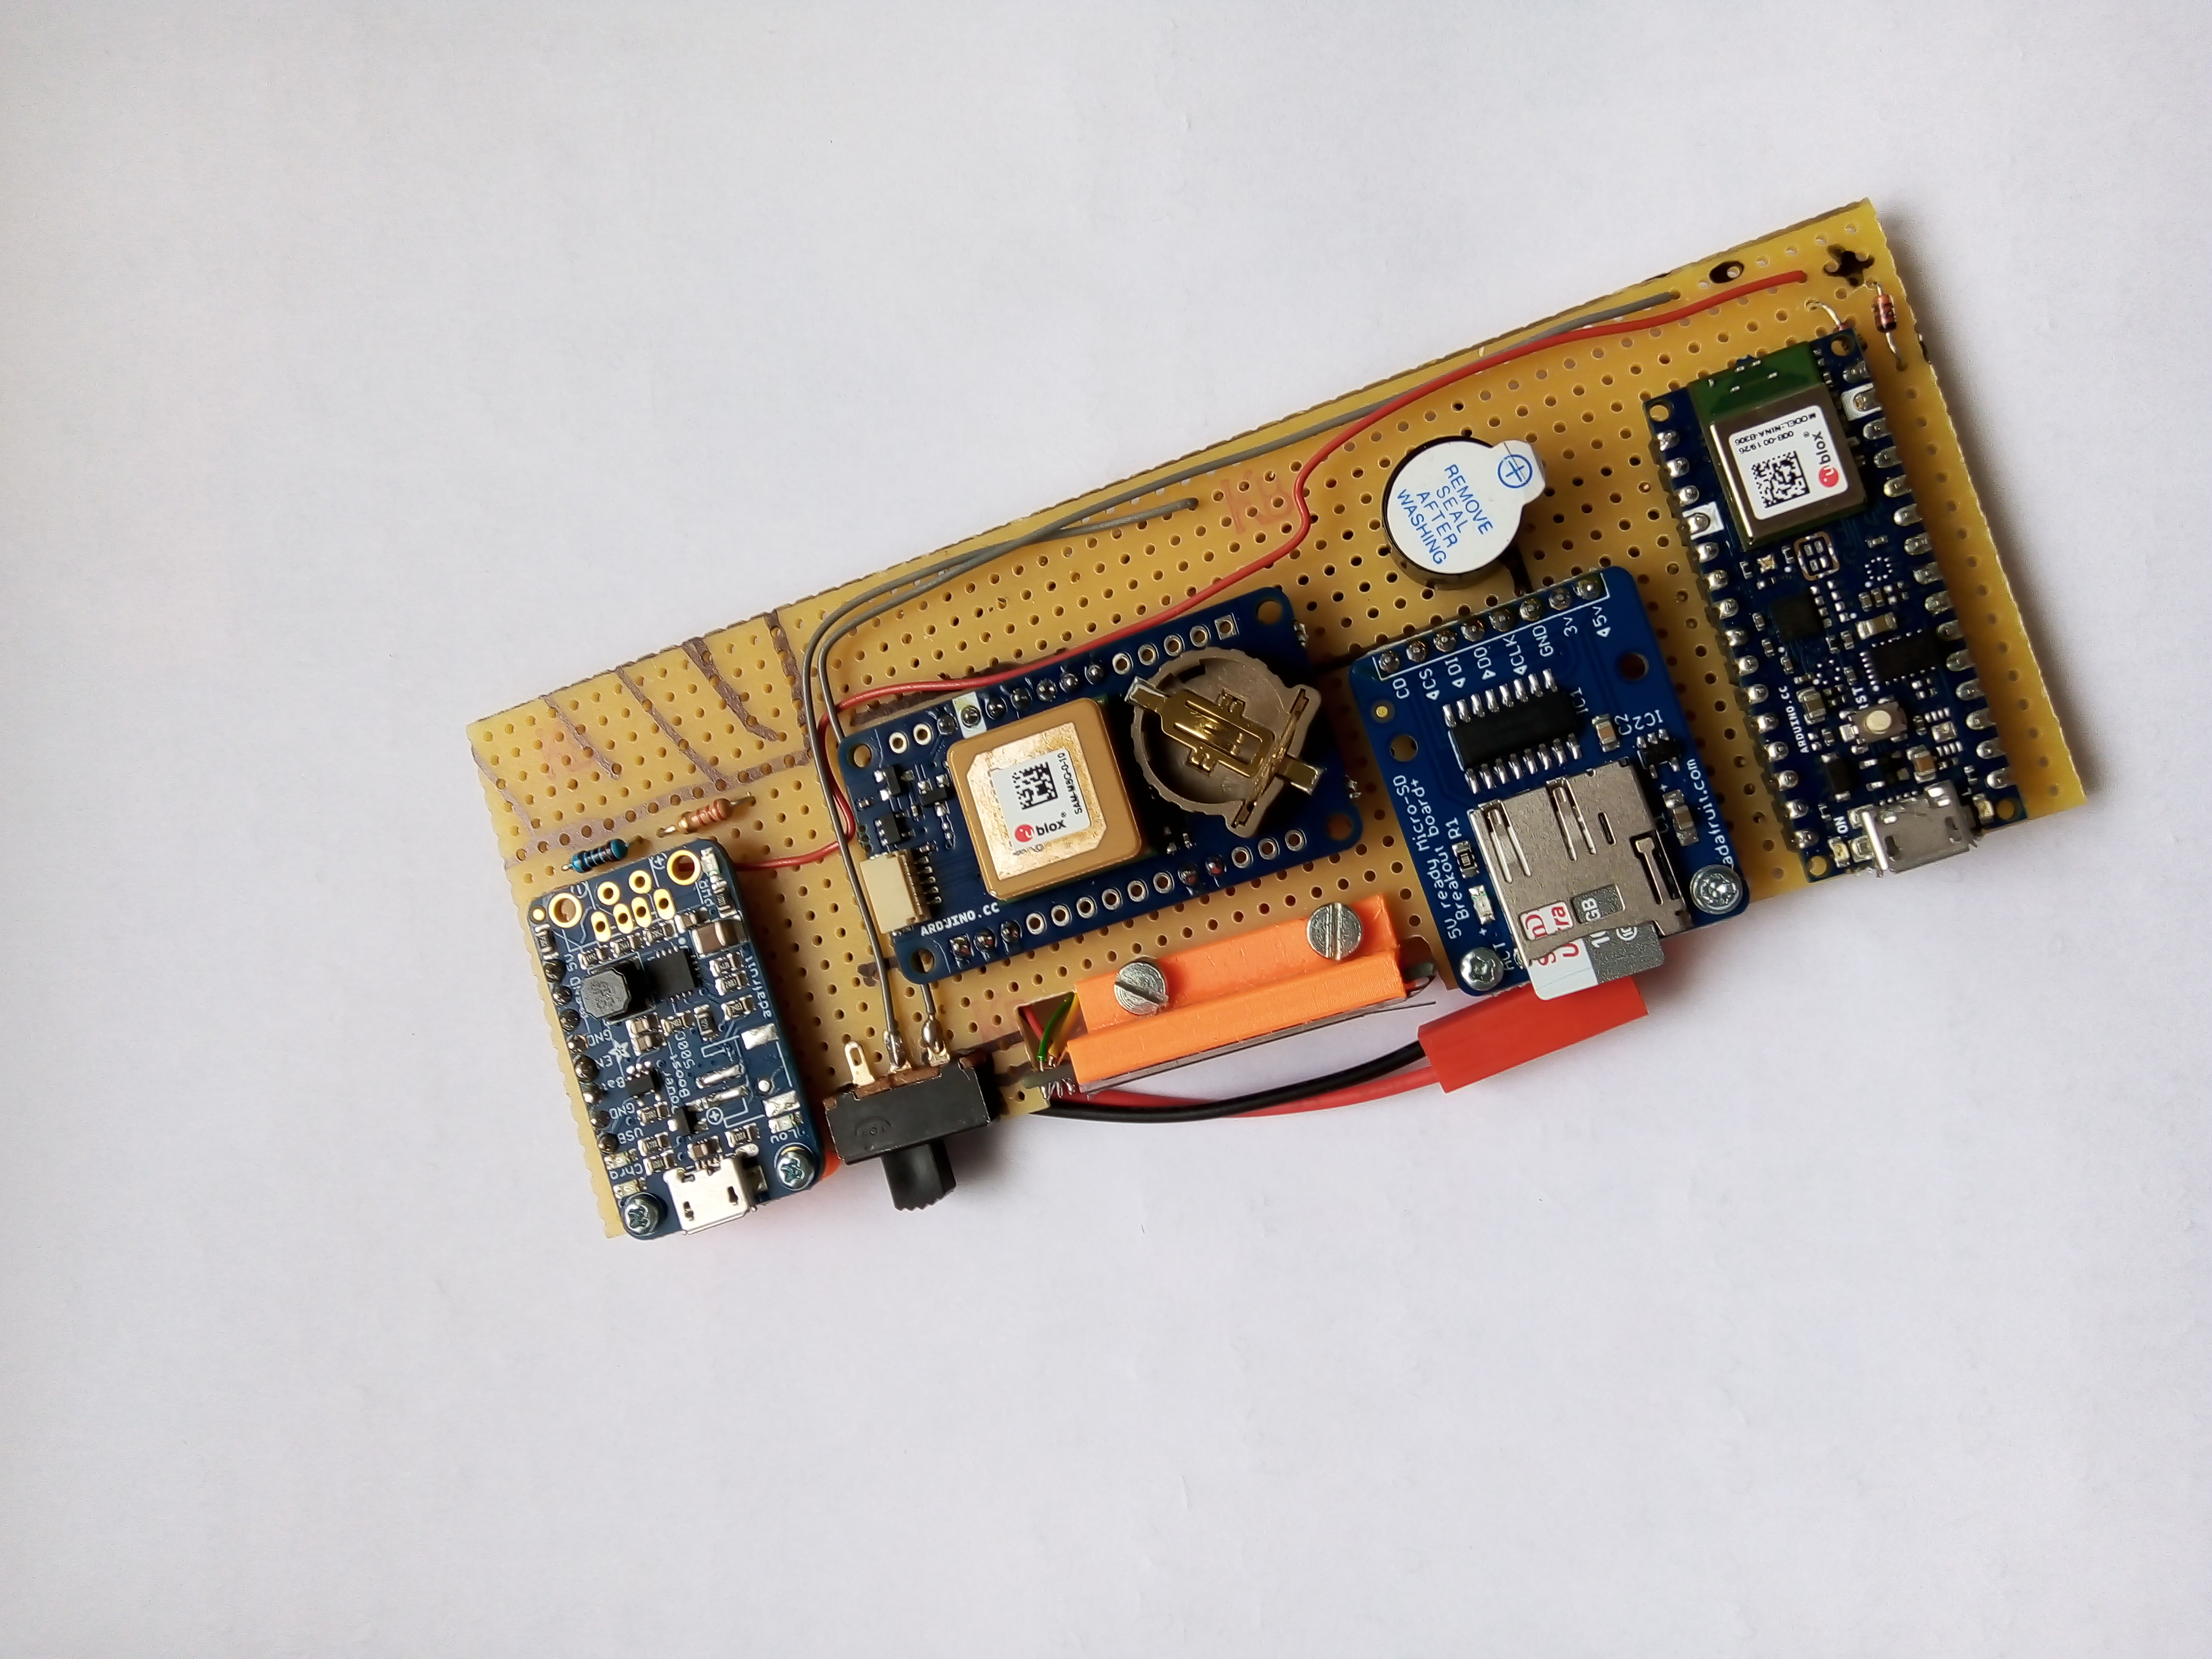
\includegraphics[width=7cm]{Figures/pcb_top.jpg}}
    \hfill
    \subfigure[]{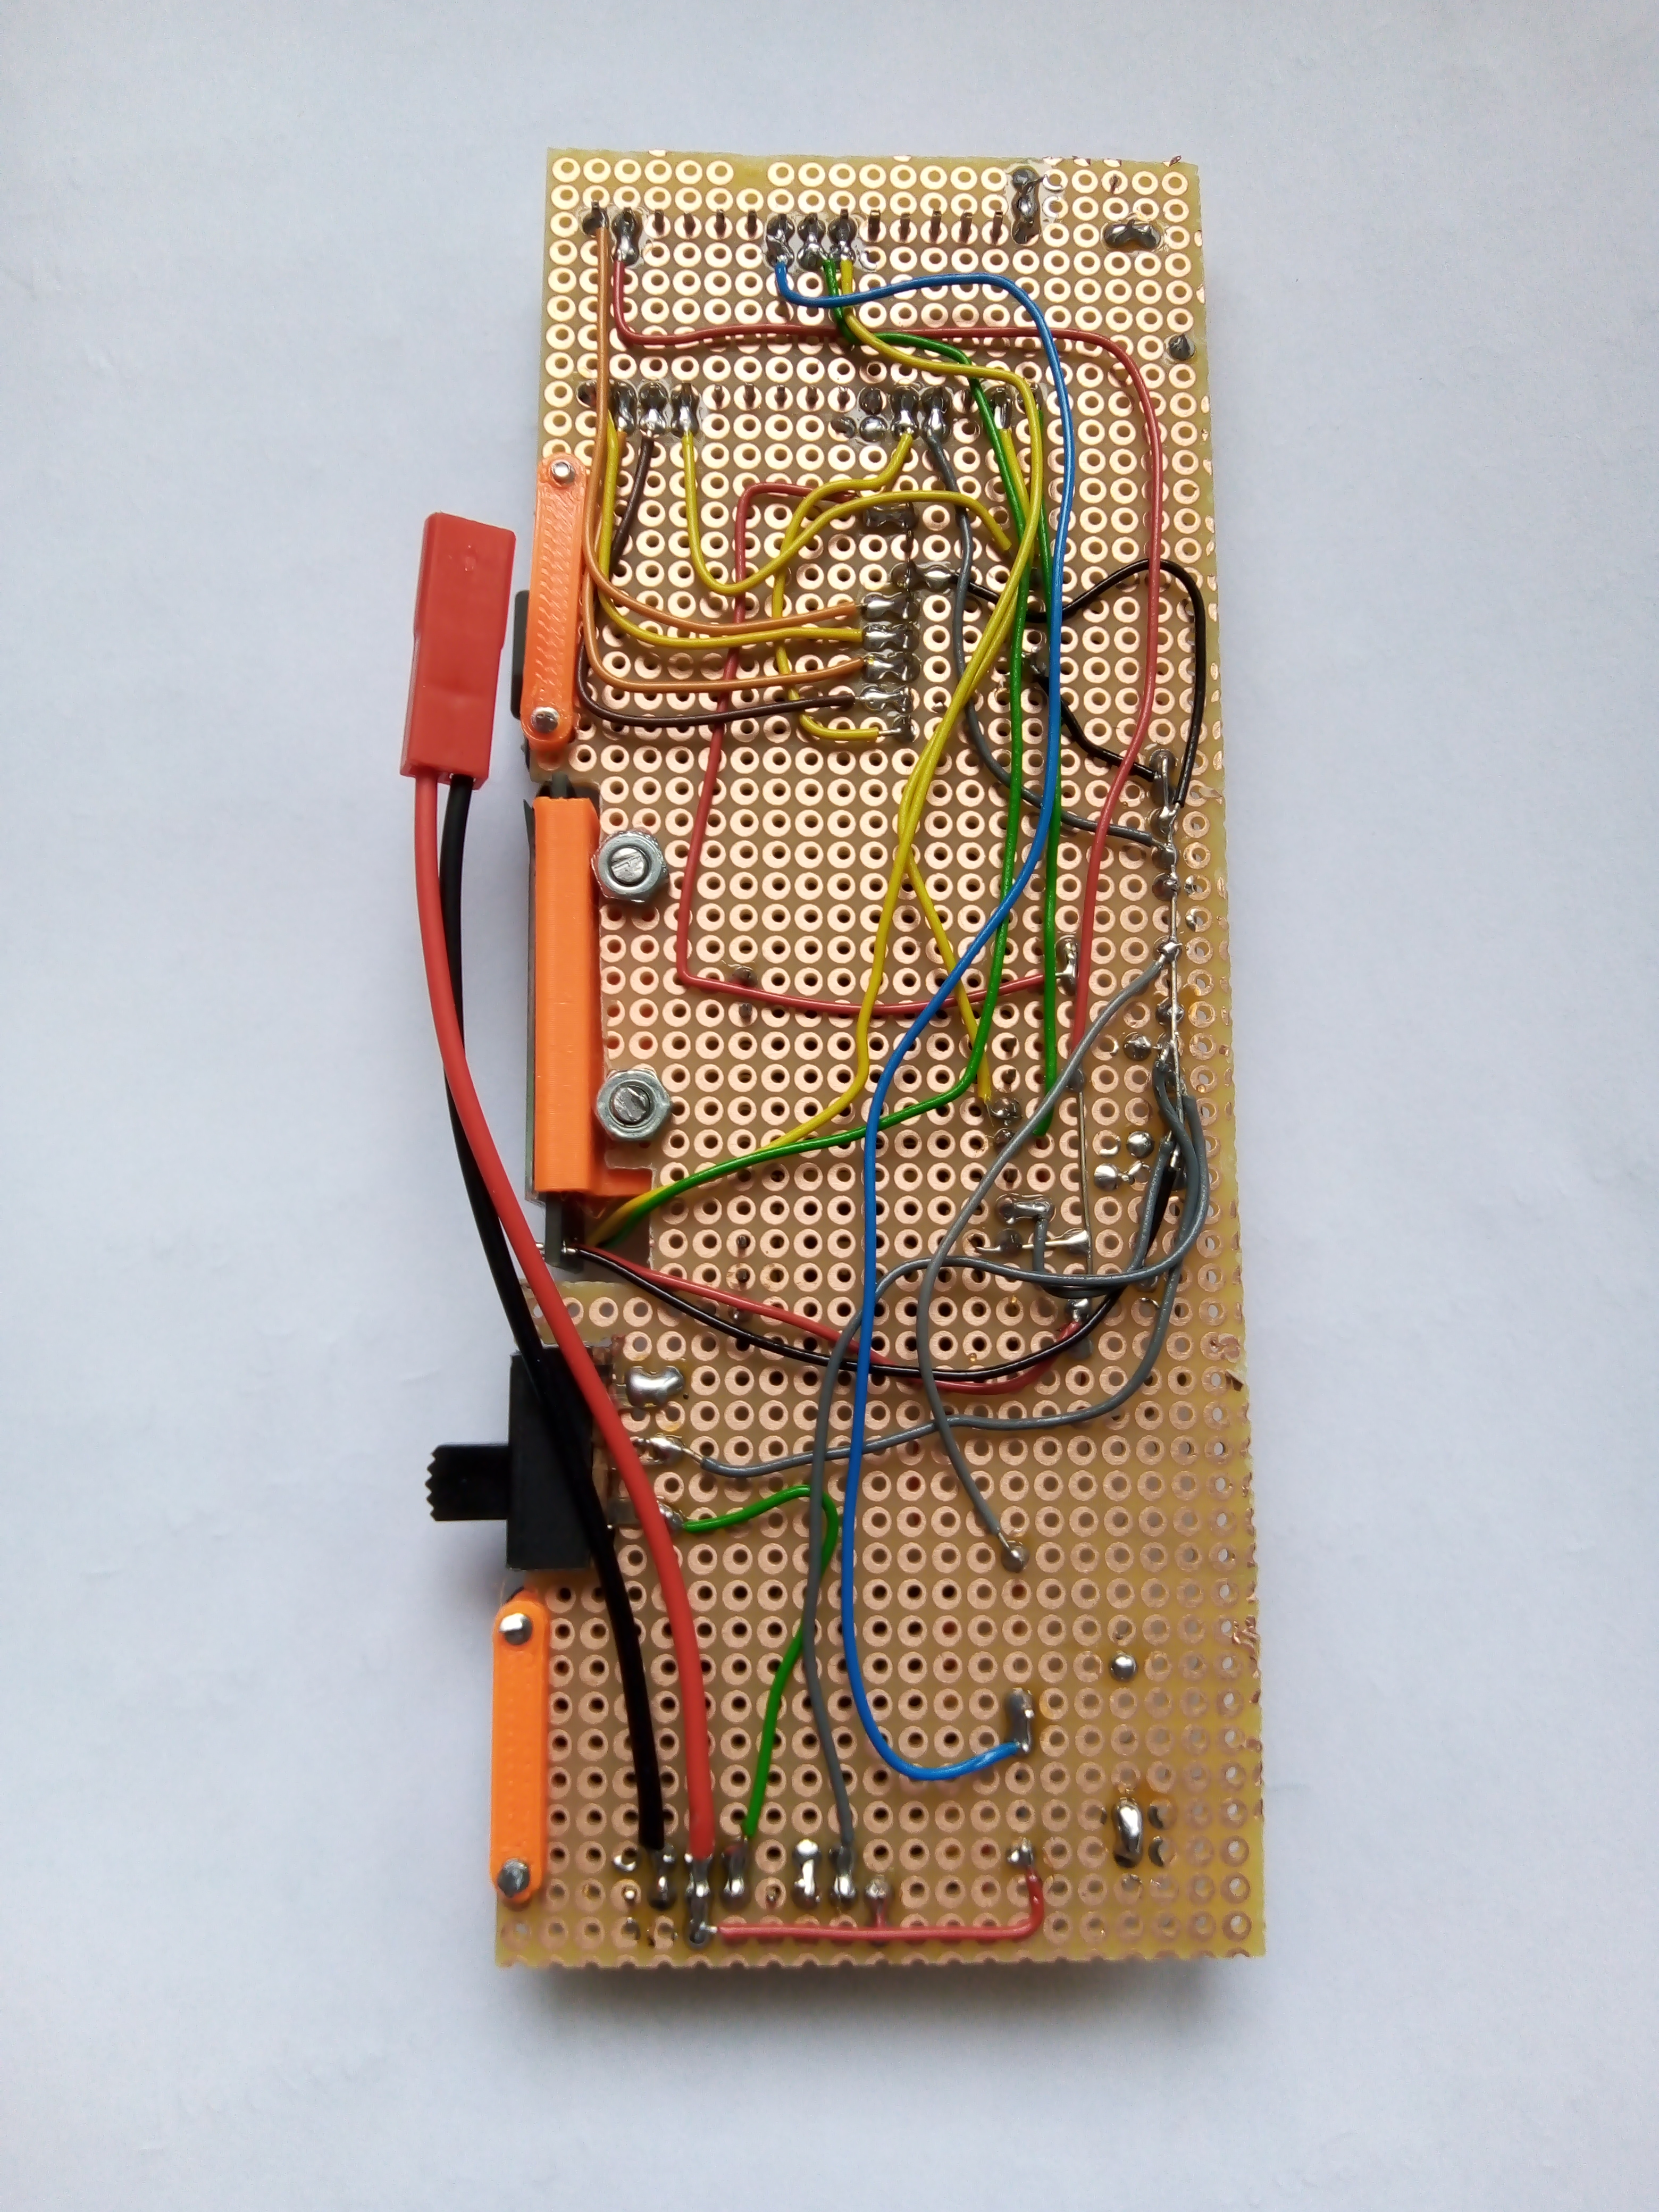
\includegraphics[height=6cm]{Figures/pcb_back.jpg}}
    \hfill
    \caption{(a) The top view of the pcb with all the components soldered on place. (b) The back side of the pcb showing how the wiring was done. All wires are single-core wires.}
    \label{fig:pcb_plain}
\end{figure}

The components in figure \ref{fig:pcb_plain} (a) are from left to right: LiPo charger/boost converter module, power switch, GPS module, OLED screen (mounted vertically to the orange holder), microSD adapter, buzzer (with the white cover still on) and the microcontroller unit. The power switch that is connected to the charger module and also to upper-right corner of the board which makes it possible to power the device from external 5-21 V power supply. When powered through that connection, the regulator of the microcontroller is used to lower the voltage to 3.3 volts. Lastly there is a voltage divider behind the charger module that allows reading the battery level with the microcontroller analog input. Now everything could be tested by simply hooking up the battery and writing a short sketch that displays acceleration and location on the OLED screen. After making sure that everything worked, it was time for the enclosure design.

The pcb measures 142x55 mm and the screen is the highest component with the height of 16 mm. This means that the enclosure could be taller and longer to fit the connectors and buttons, but the width was quite close to maximum. After a bit of drawing and modelling, the enclosure design was obtained: The external sensor connectors are mounted to the microcontroller end and the two user interface buttons (navigate and select) were mounted on the side and there was a small cutout made to the upper-left corner of the pcb to fit the buttons without making the enclosure wider. The dimensions of the enclosure are 180x68x28 mm and it is designed to be mounted to the down tube of the bike, ideally using water bottle mount to secure it on place. The Solidworks model of the enclosure is shown in figure \ref{fig:enclosure_CAD}.

\begin{figure}[H]
    \centering
    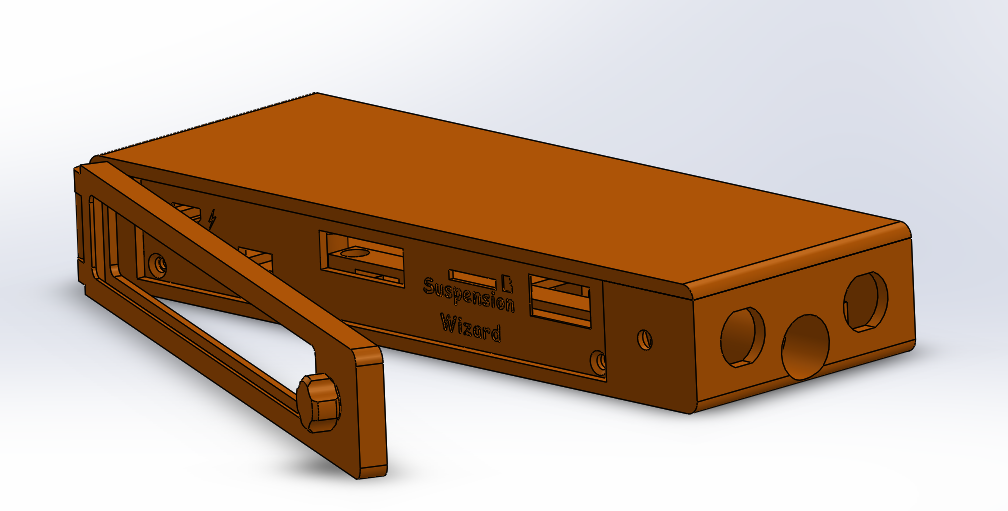
\includegraphics[width=100mm]{Figures/enclosure_assembly.png}
    \caption{Solidworks model of the assembled enclosure.}
    \label{fig:enclosure_CAD}
\end{figure}

The enclosure consists of four parts: The main part, top cover, door and front plate. The main part and top cover form 5 sides of the enclosure and the door with a plexiglass window is attached to the side on which the OLED and power switch are located. This allows the enclosure to be watertight while you can still read the display and navigate with the buttons. The front plate covers the electronics behind the door. The reason for not printing the front plate directly to the main part is that this way the electronics can be upgraded in the future and the same main enclosure can still be used with just a new front plate. The figure below shows the enclosure and the final circuitry with all the buttons and connectors soldered on place. The LiPo battery is mounted underneath the pcb on to a 3D printed cage that is bolted to the bottom of the main part.

\begin{figure}[H]
    \centering
    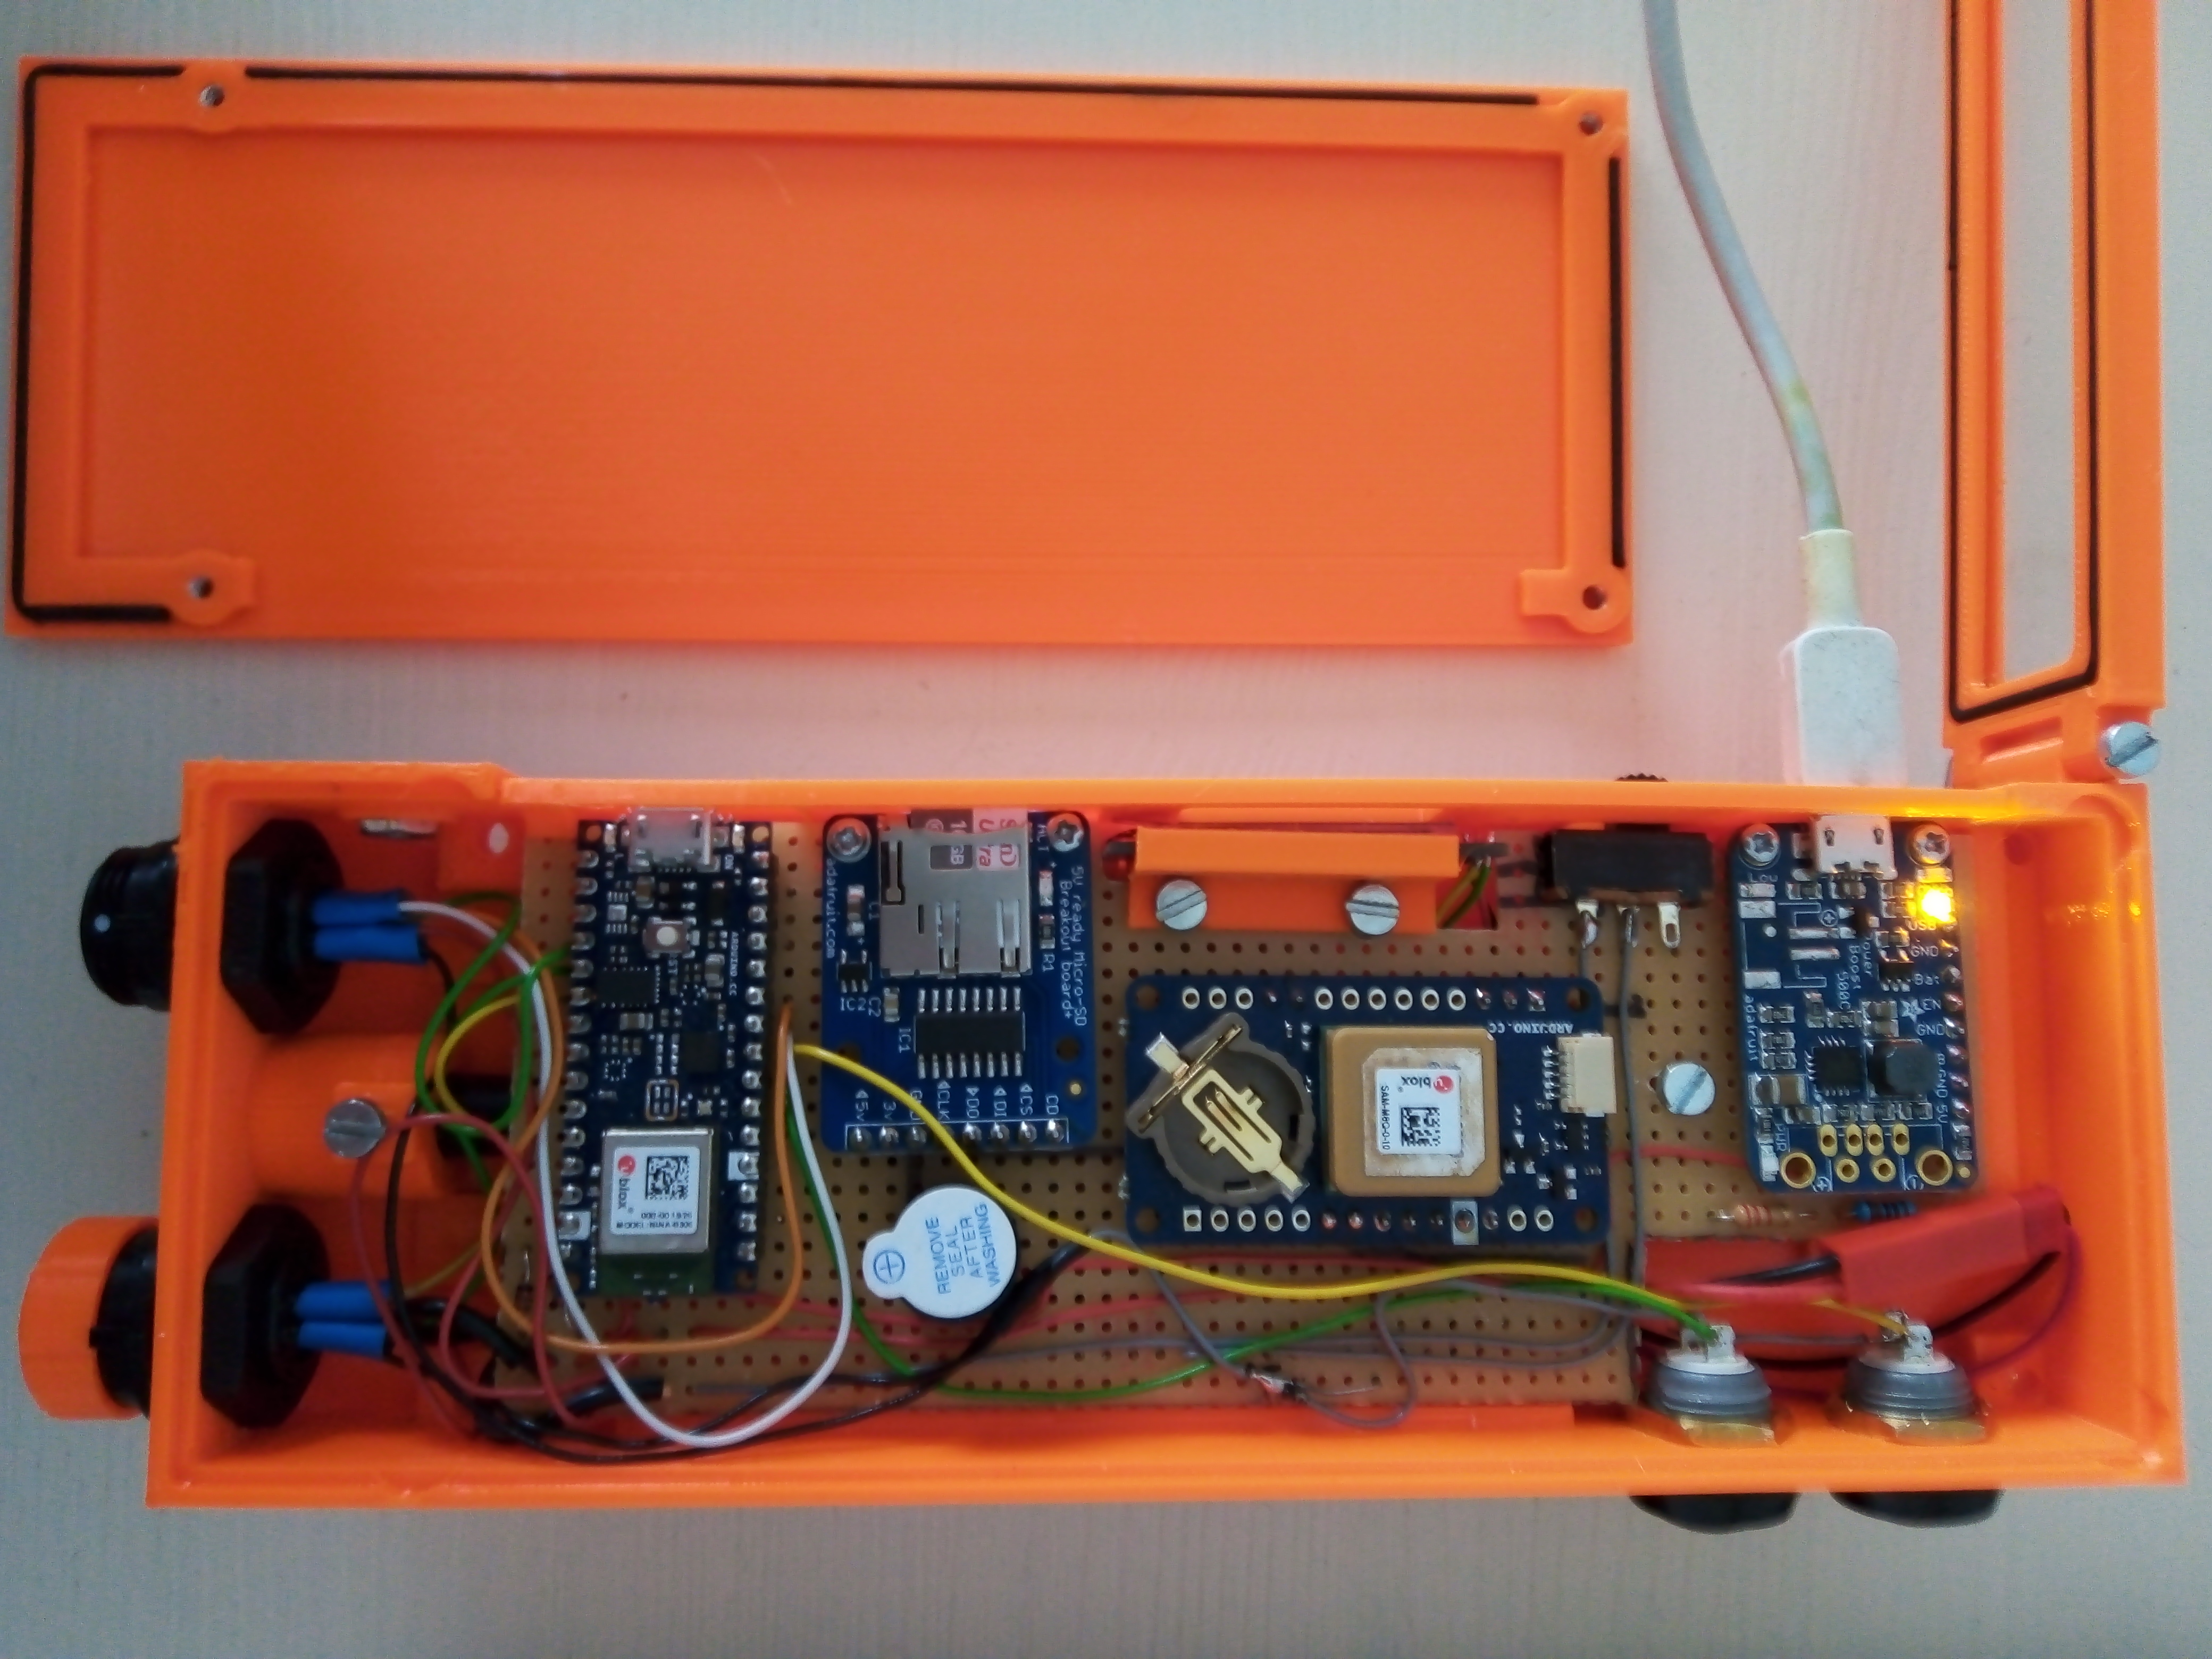
\includegraphics[width=100mm]{Figures/measurement_unit.jpg}
    \caption{The finished main unit with the top cover removed. The seals of the enclosure door and the top cover can be seen easily this way.}
    \label{fig:enclosure_opened}
\end{figure}

The water-tightness of the enclosure was further enhanced with using some seals made out of O-rings to seal the door and the top cover to the main part. In figure \ref{fig:enclosure_opened} above there is an orange cap on the other sensor connector. The cap is used cover the rear shock sensor when measuring bikes that don't have rear suspension. Between the sensor connectors there is a male DC21 jack that can be used to connect regular bicycle light battery to the device.

Now when the mechanical design and electronics were ready it was time to start programming. The plan was to implement a simple user interface that works with the push buttons and displays menu on the OLED screen. The code structure follows object-orientated programming as it consists of two c++ classes, Menu and Measurement. The Menu class runs the user interface and uses a switch-case structure to determine which screen to display. From the menu the user can calibrate the device, scan memory card for saved trails, adjust bike specific settings and start measurements. The Measurement class is the one that interfaces with the sensors and runs the measuring events. One issue that came up when testing the components separately was that the GPS update rate is quite low and it would kill the sample rate of the device. The Mbed RTOS gives a potential solution to this problem as you can start multiple threads and specify their priorities. So by running sensor polling in separate thread and specifying its priority higher than the GPS thread, it should be possible to crank up the sample rate. The reason why GPS isn't so important is that it is anyway so inaccurate that it is enough to get location only once every second. 

The programming phase introduced many challenges as the threads and interrupts didn't play along very well. The things that didn't work were interrupt detaching and re-attaching and terminating and starting thread again. After modifying the code so that the ok-button measurement stopping interrupt didn't have to be detached, the device didn't jam, when starting second measurement after power up. The problem was still that the measurements after the first one recorded only constant values. This was caused by the fact that threads were declared as global variables and re-started for every measurement, which some how didn't execute the polling task. Changing the threads to local variables fixed this bug. The sample rate issue wasn't solved with thread priorities, but with sd card usage. The first version of the code flushed the data to the card between every sample and this was very slow as each flush takes about 180 ms. When the flush rate was altered, the sample rates were greatly improved and the finished device can measure up to 180 samples per second with GPS and over 350 samples without GPS. The higher number of writes between each flush means that the risk of losing data is higher, but testing hasn't yet shown that this would be significant as there has been no sign of lost data.

Final touches to the Arduino code were that the flush rate was implemented to be user configurable e.g. the user can in theory adjust the sampling rate through the flush rate as they have some what linear dependency: flush rate 1 → sample rate 4 Hz, flush rate 200 → sample rate 350 Hz. Another feature that was added was adjustable measurement filtering with running average, that is taken care of by Average class. This means that the user can specify the buffer length for the running average and this way either filter the data on board or record raw data and filter it in the analyzing phase. The data review without laptop was set to be one of the requirements and on the microcontroller end it is implemented using one BLE service with 10 characteristics to represent the data. The calculated values are average used travel f/r, maximum used travel f/r, highest compression and rebound speeds f/r, brake usage and elapsed time. The speeds are obtained through numerical differentiation and the brake usage is calculated by comparing the number of sample points to the number of points when at least one brake was being used. The phone app is causing a bit problems as the MIT App Inventor BLE extension seems to not be able to listen multiple characteristics simultaneously. The status of the app is shown below in figures \ref{fig:MIT_app} (a) \& (b): It receives data only trough one characteristic and it's meant to subscribe/unsubscribe the values, when timer ticks, but that isn't some how working as the recieved data isn't changing.

\begin{figure}[H]
    \hfill
    \subfigure[]{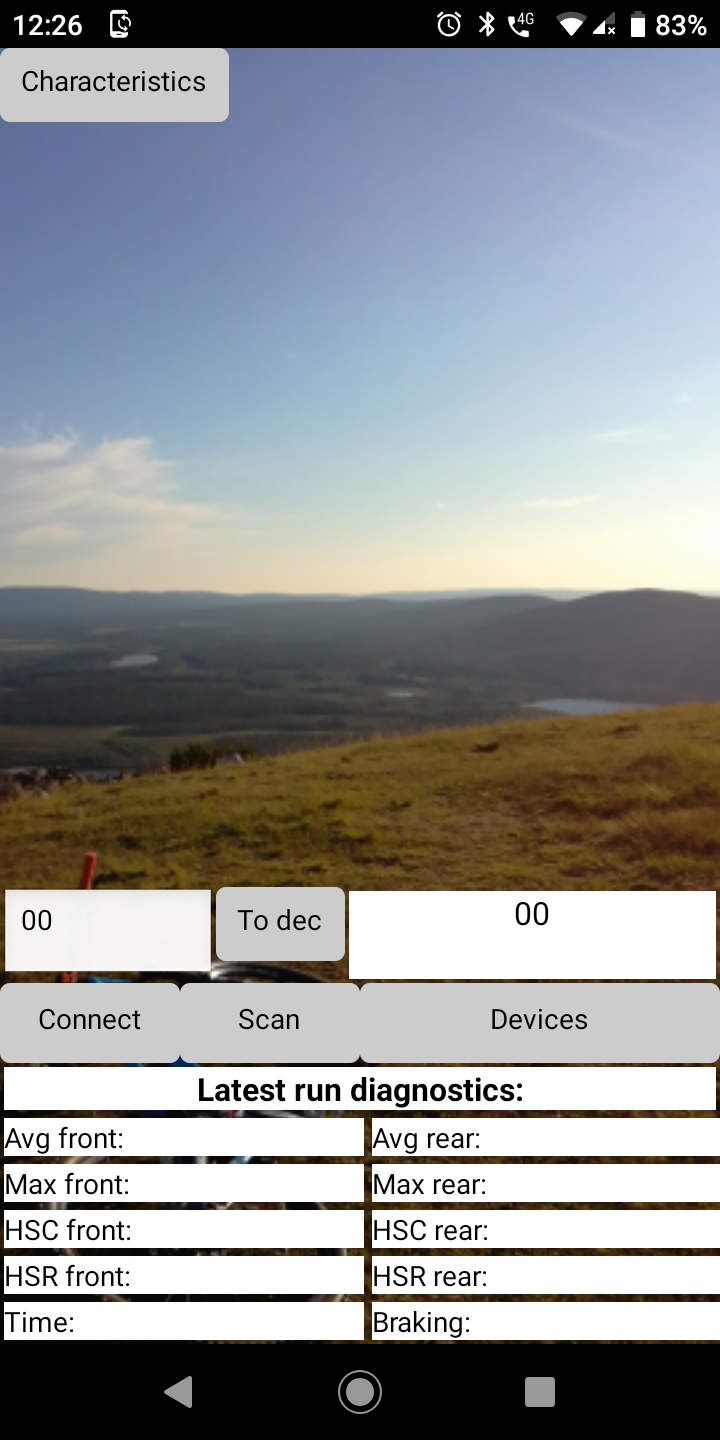
\includegraphics[height=8cm]{Figures/app_screen.png}}
    \hfill
    \subfigure[]{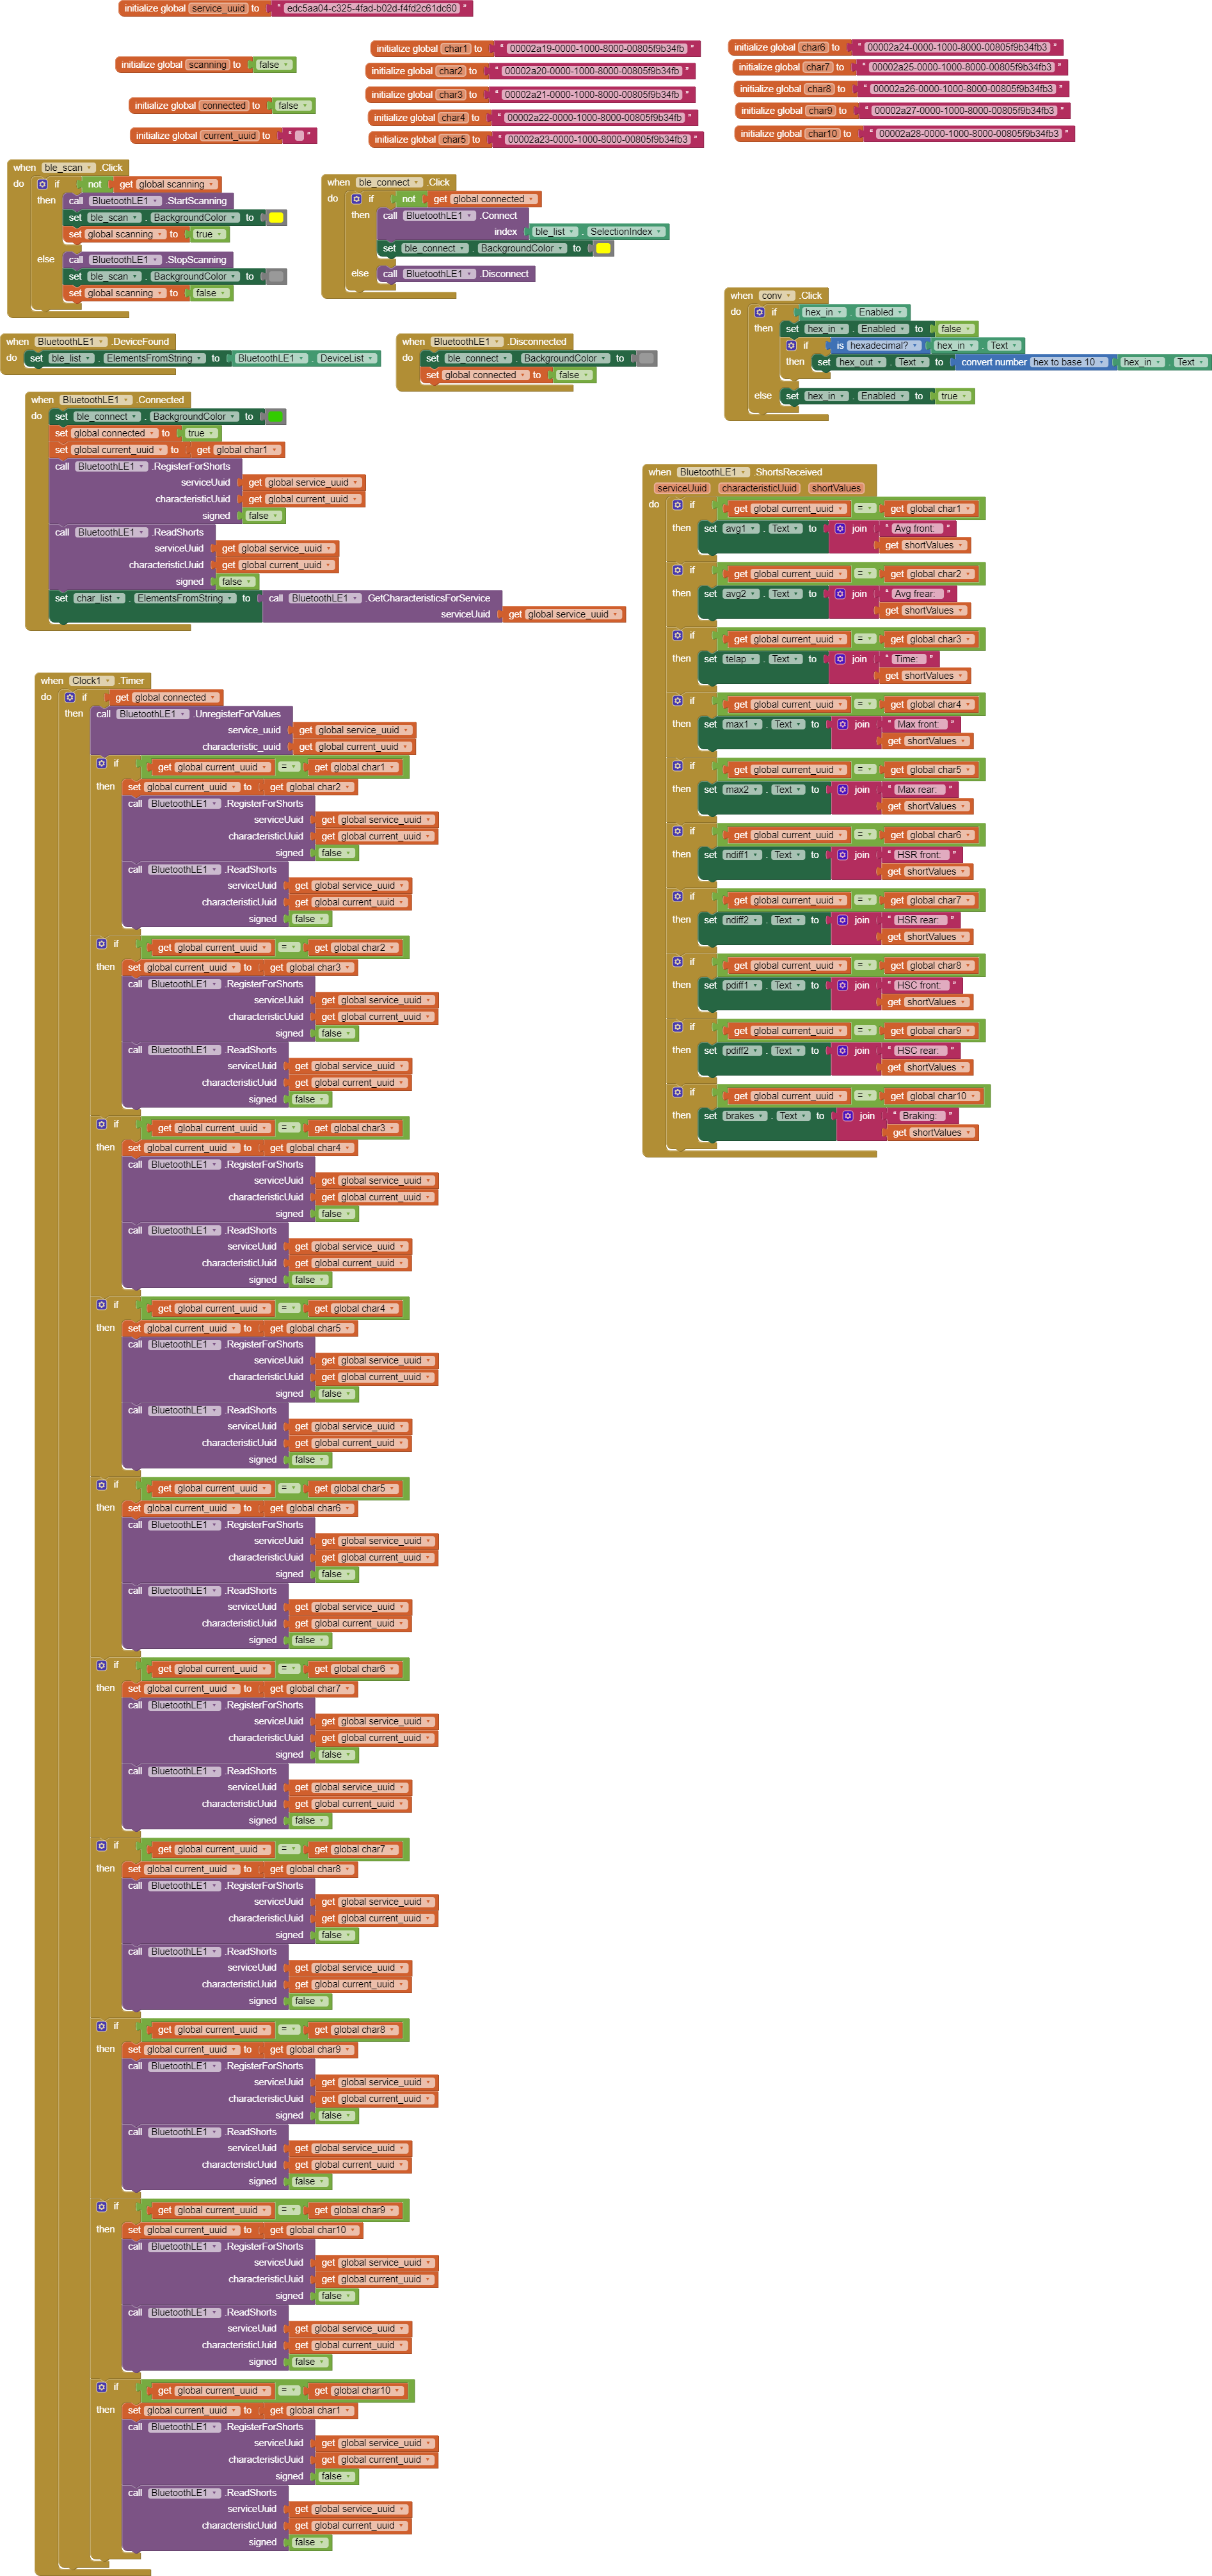
\includegraphics[height=8cm]{Figures/blocks.png}}
    \hfill
    \caption{(a) A screenshot of the phone app. (b) The blocks used in the MIT App Inventor code.}
    \label{fig:MIT_app}
\end{figure}

This means that the data review can be done with BLE terminal app or with Adafruit's Bluefruit connect app. The conclusion section will consider this topic more deeply, but it can be said that WiFi would have been better wireless communication option for the project in terms of usability from the end user's perspective. The source code for the whole project can be found from the \texttt{Arduino code} folder of the repo.

Figures \ref{fig:all_parts} (a) \& (b) below show all parts of the device: Figure \ref{fig:all_parts} (a) one has the external sensors and the mounting hardware. The small roller wheel on the down-left corner is meant for mounting flexibility: If there is not enough space or the mounting would be difficult, the rear sensor can be mounted to the frame and the string is guided through the roller. This should be useful on four-bar linkage design bikes as the rear sensor enclosure can't be attached to the rear shock or to the main link, so the sensor can be attached to the downtube and the roller to the lower shock mount. In figure \ref{fig:all_parts} (b) there is the main unit and three different mounting solutions, which are Fidlock magnetic water bottle mount, 50 mm diameter round cable tie mounts and cable tie mounts for triangle-shaped frame tubes.

\begin{figure}[H]
    \hfill
    \subfigure[]{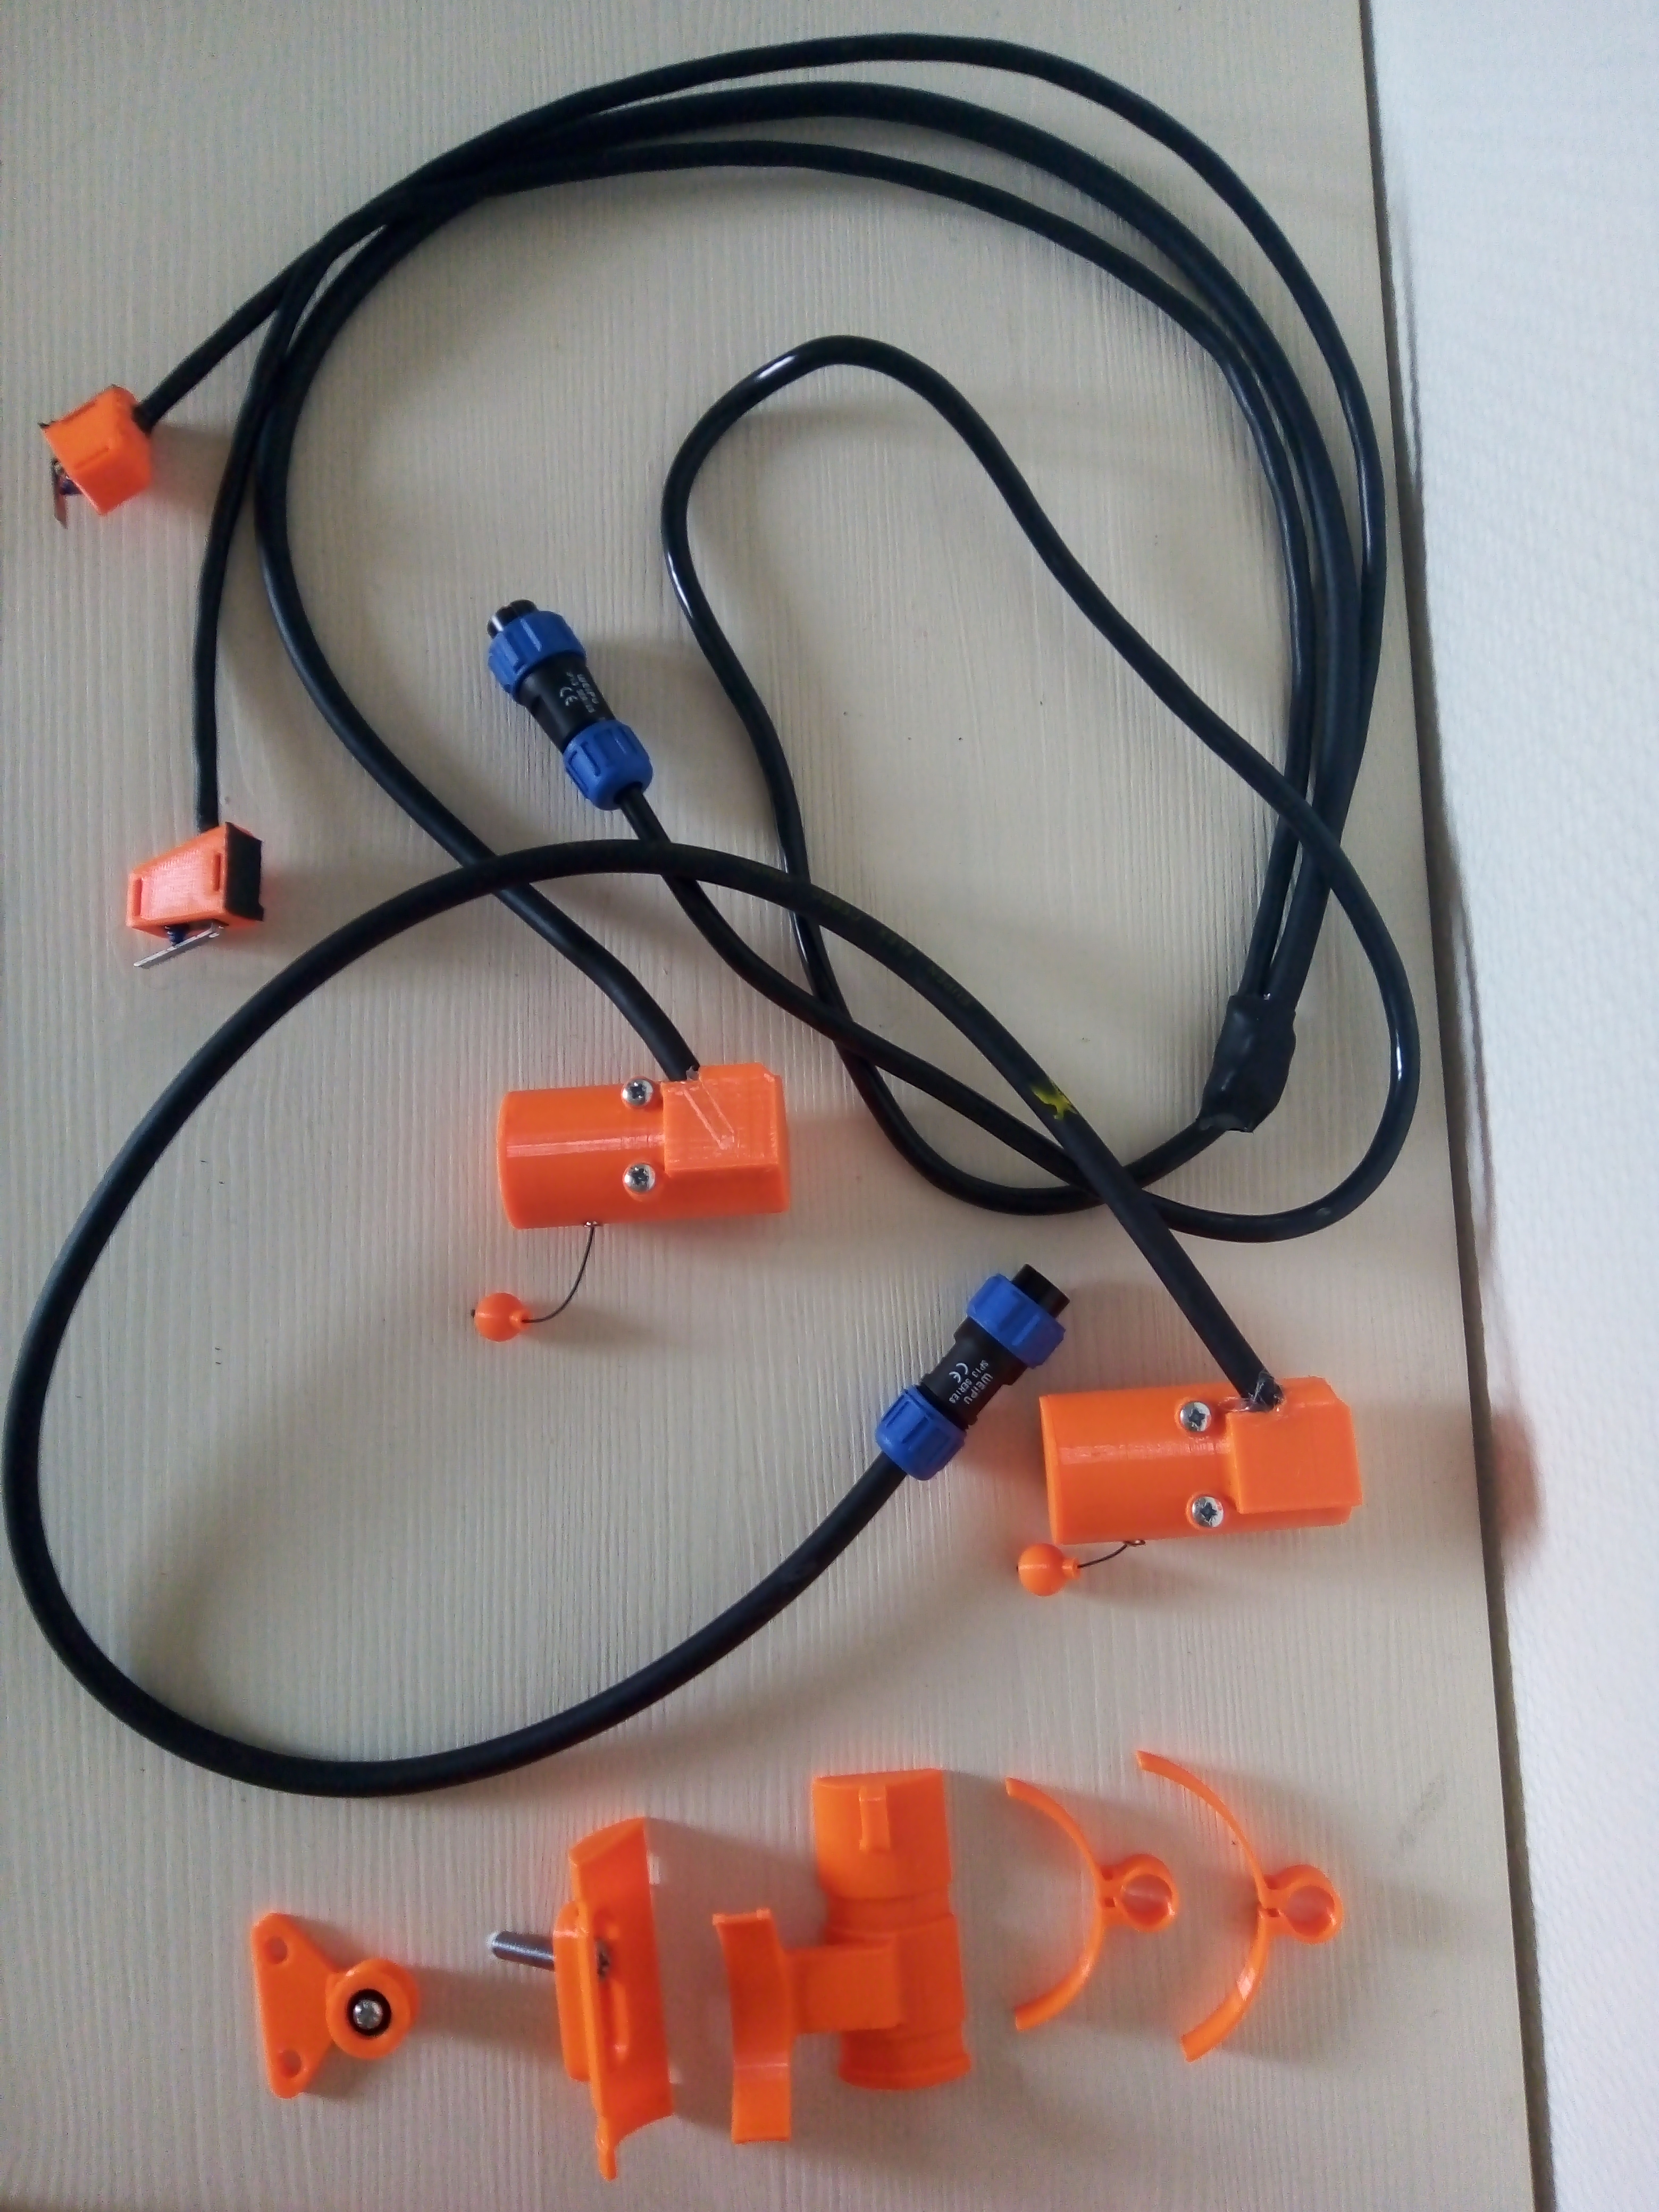
\includegraphics[height=7cm]{Figures/osat_2.jpg}}
    \hfill
    \subfigure[]{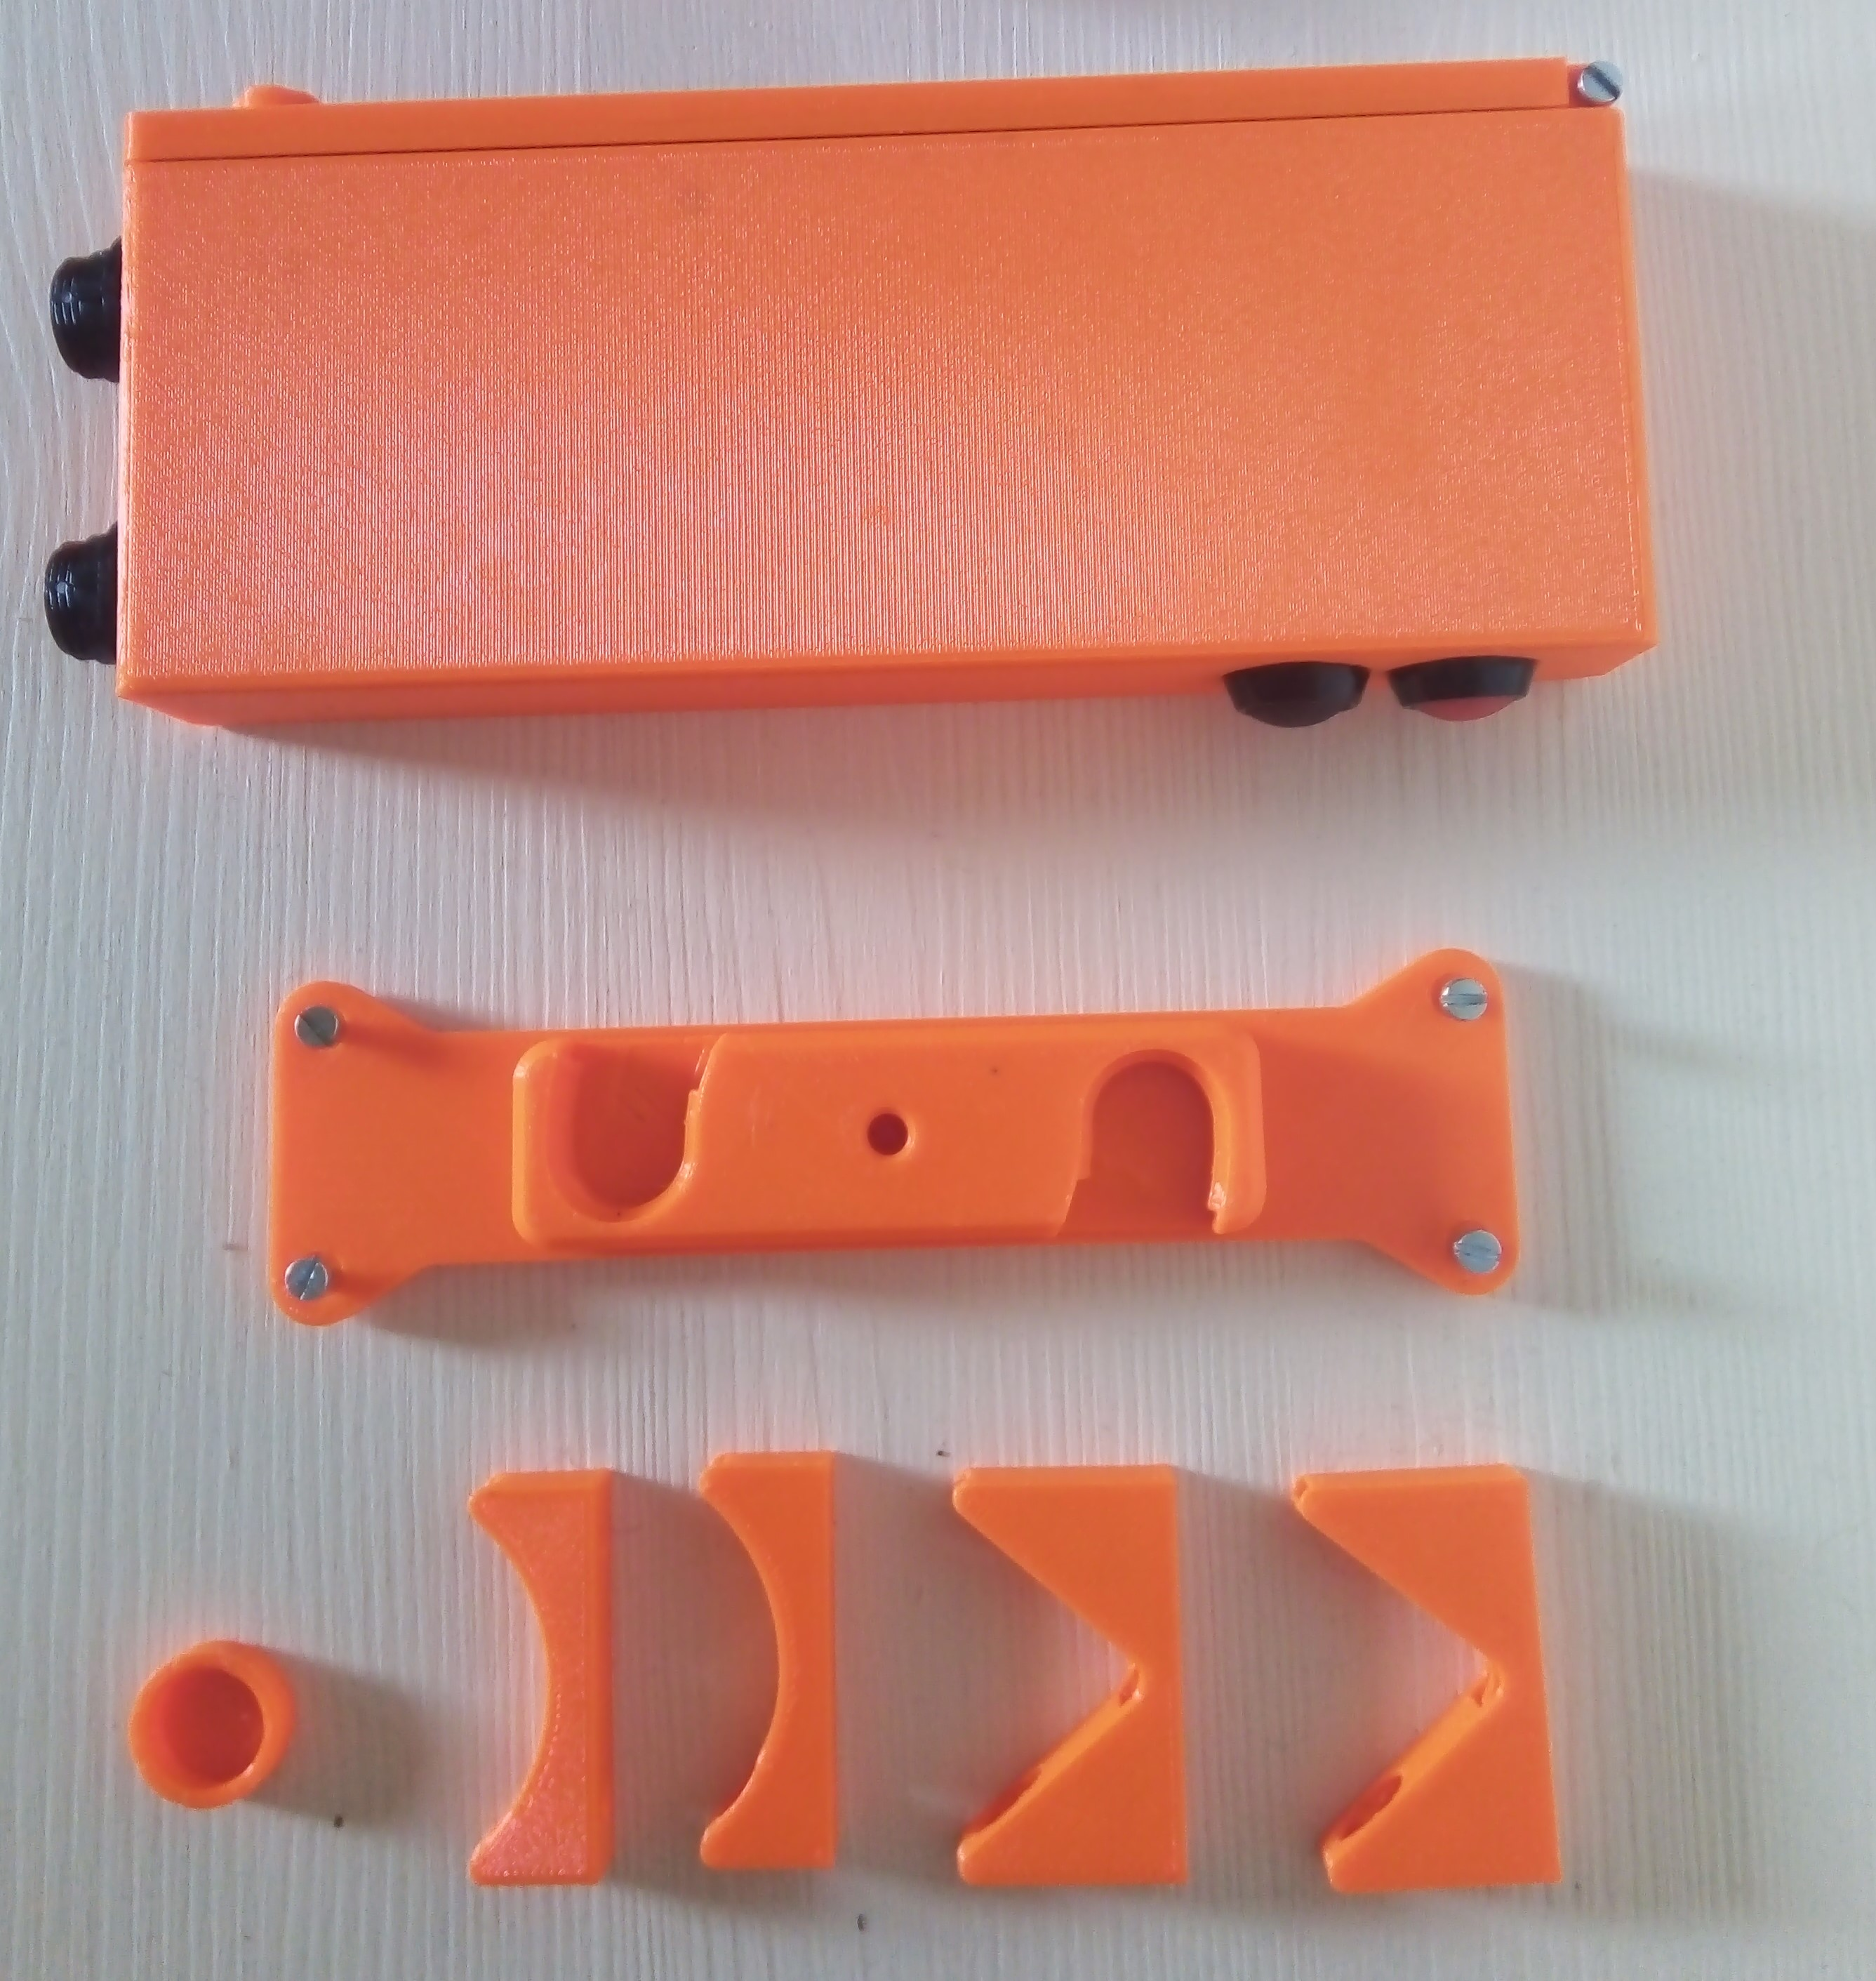
\includegraphics[height=7cm]{Figures/osat_1.jpg}}
    \hfill
    \caption{(a) The external sensors and their mounting hardware. (b) The main unit and its mounting solutions.}
    \label{fig:all_parts}
\end{figure}



\newpage
\section{The result}
\rule{12.7cm}{0.4pt}

\subsection{Description of the device and its uses}

The meaning of the project was to make a cheap mountain bike suspension data logging system that could be used by average mountain bikers. The idea is that this way the mystery of good suspension setup could be examined and studied by more people than the world cup racers who have access to measuring devices that cost 10 times the budget of this project. One could think that this kind of device is only useful for racing purposes, where being faster is the only goal. This isn't the case though, as a rider can also use this device to learn about one's riding style and suspension usage and this way obtain a better suspension setup (or conclude that current one is perfect). This matters a lot as the riding experience can be totally different when the bike is working properly, as the riding will feel easier and offer more fun. Potentially even beginners who have problems figuring out the correct setup could use this kind of device to speed up the adjusting process. This case is actually quite relevant as the increasing popularity of mountain biking means that bikes are getting cheaper and nowadays even entry level bikes have so much adjusting options that one can easily get carried away with those.

What does the device give then? It gives damper shaft position data, braking data and accelerometer data that can be used to study the behavior of the suspension. For instance, the correlation coefficient between damper position and z-direction acceleration of the frame gives some hint about the damping performance (on a full suspension bike, on a hardtail the acceleration tells how big shocks the rear wheel has taken). The brake data can be used to study how the suspension works under braking: Most designs cause torque, which makes the suspension less sensitive under braking. Finally, to be able to backwards correlate all the data, the on board GPS records the location and speed. The figures \ref{fig:data_plots} (a) \& (b) show recorded data from a winter trail in Espoo, the bike ridden was a hardtail meaning that it had only front suspension.

\begin{figure}[H]
    \hfill
    \subfigure[]{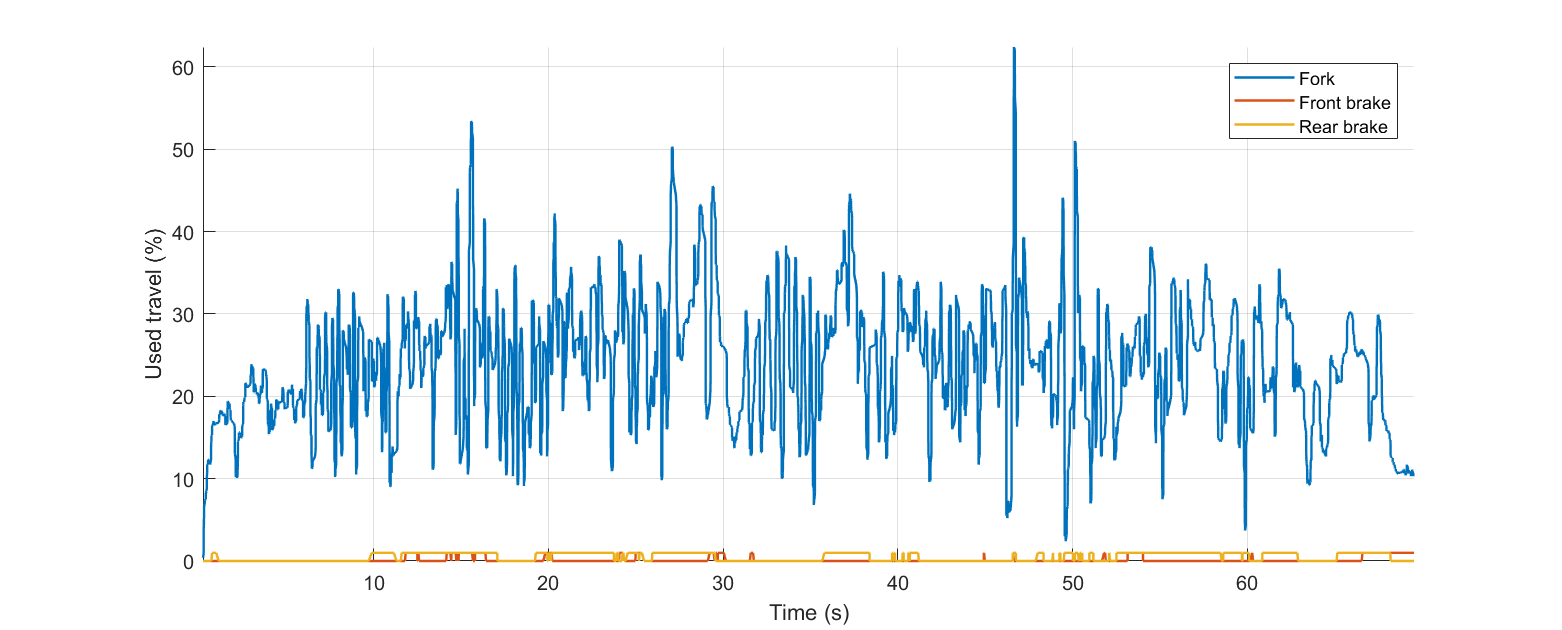
\includegraphics[width=6.2cm]{Figures/hardtail_run.png}}
    \hfill
    \subfigure[]{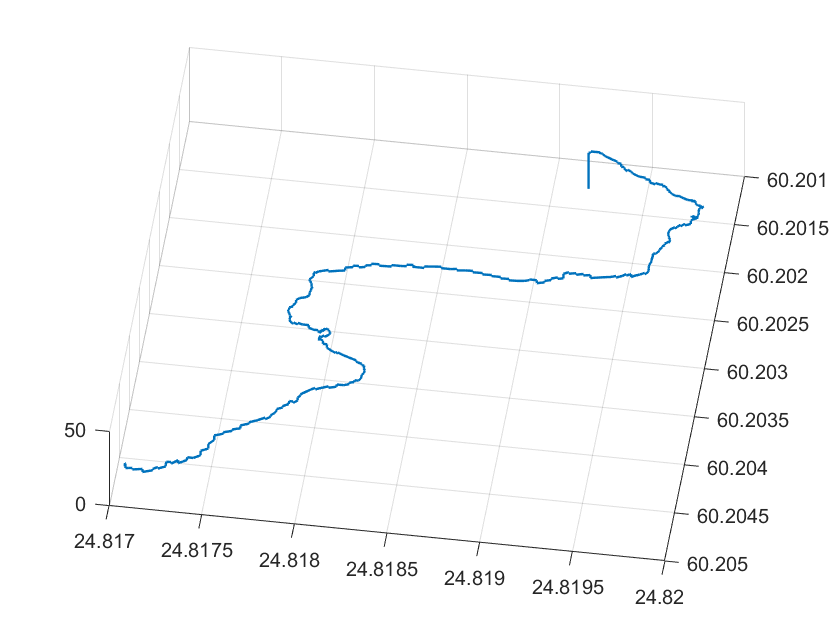
\includegraphics[width=6.2cm]{Figures/gps_3d.png}}
    \hfill
    \caption{(a) The fork travel usage as a function of elapsed time [s]. (b) A visualization of the GPS tracked path.}
    \label{fig:data_plots}
\end{figure}

Figure \ref{fig:data_plots} (a) tells that on average the used suspension travel was around 25\% and the maximum was 63\% (when landing a jump). Based on those one could argue that there was too much air in the damper (air works as the spring in the used fork), but if there were thermometer data the result would have natural explanation as the damping oil meant for summer conditions is too viscous in -15°c temperatures and the system is over damped. Figure \ref{fig:data_plots} (b) shows the route that was ridden and by labeling that with different values, for instance speed, braking or suspension usage, one can easily find out the behavior of the bike on different sections of the trail. A better results analysis code implemented using Python can be found from \href{https://github.com/valtttu/DIY-suspension-wizard-data-analysis}{github.com/valtttu/DIY-suspension-wizard-data-analysis}.


\subsection{Presentation/demo video}

The video behind the link below goes trough some basic info about the device and shows how to record manually. The bike used in the video has same fork travel and rear shock stroke as the defaults of the device, so it doesn't go through changing those. Those can be changed from the settings menu, where the 'use gps option' is located.

\href{https://drive.google.com/file/d/168bjvY0lNAx_l6pTAgVNn_BvS3w7V0ZD/view}{Project video on Google Drive}



\subsection{Quick user manual}

\begin{figure}[H]
    \centering
    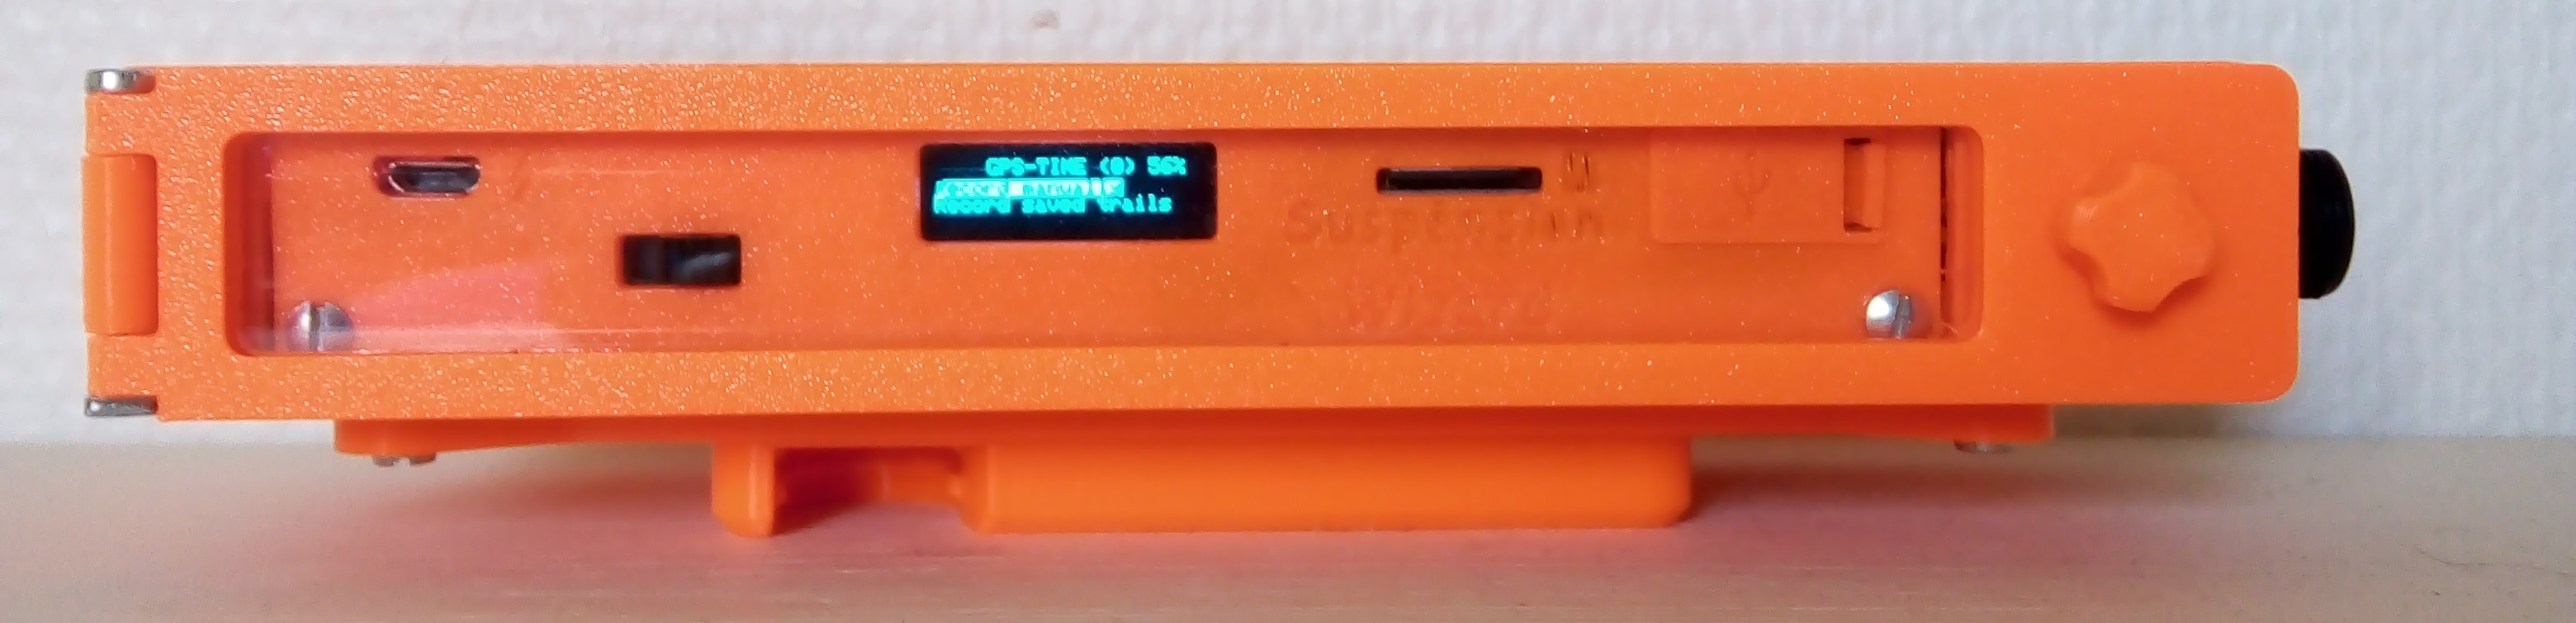
\includegraphics[width=115mm]{Figures/enc_2.jpg}
\end{figure}

This section describes how to use the device and what things should be taken into account (which parts aren't foolproof). First mounting the device:

\begin{itemize}
    \item The linear sensors (string pots) should be mounted so that the the string gets shorter when suspension is compressed. The accurate mounting solution depends on the bike, especially when considering the rear sensor as there are nearly zero identical bike designs. Best way is to manufacture a custom mount for the used bike, for instance via 3D printing.

    \item The brake sensors should be secured to the brake lever body with cable ties. In this phase, it is good to leave them a bit loose so that you can adjust the position in the calibration phase, if needed.

    \item The main unit is easy to mount to a Fidlock magnetic water bottle mount with the adapter. If this is not possible, then it can be mounted with cable ties and the adapters that bolt on the bottom of the main unit.

    \item Finally it is good to make sure that the wires don't get caught to anything while riding. This can be done by using some Velcro tape to secure the wires to the frame tubes.

\end{itemize}

Next up the user interface navigation for setup. The device doesn't have on board non-volatile memory for saving settings, which means that the initial setting and calibration procedure needs to be ran every time after starting the device. The procedure has following stages:

\begin{itemize}
    \item Power up the device from the power switch.

    \item If something goes wrong in the booting phase, an error will be thrown to the OLED screen. If this happens, toggling the power switch might help or if the error has something to do with the microSD, you can try to remove and install it again.

    \item Navigate to settings menu. 
        \begin{itemize}
            \item Set your bike specific fork travel and rear shock stroke length. The defaults are 160 mm and 57 mm.
            \item In case you are measuring full suspension bike and didn't have the rear sensor connected when powering up the device, choose the 'Add rear sensor' and the device will detect the rear sensor. This is done automatically, if the sensor was attached before powering up the device.
            \item If you are in an area where getting GPS signal is tricky, you can disable GPS by setting the 'Use gps option' to false. Note that the automatic recording needs GPS to work so by setting this option to false, only the manual recording will work.
            \item Change the sample rate (microSD flush rate, see programming section (end of 3.1) for more info) and running average sampling length if you want to. Defaults are 200 and 5.
        \end{itemize}

        \item Exit from settings menu and go to calibration menu and choose 'Calibrate all'.  Follow the instructions on the OLED screen and the device guides you through the calibration process.

        \item After calibration you are ready to record manually, but for automatic recording there is one more thing that must be done. If you have uploaded gpx-files with track segment to the microSD, you should choose the 'Scan for trails' option in the main menu. Then device will try to extract the start and endpoints of those segments from the files. This will take some minutes and after the scan finishes the device tells the number of valid trails found. Note that the gpx-file should contain only the track segment and it should be located in "\textbackslash trails\textbackslash" directory on the microSD.

        \item Now you are ready to start recording.
\end{itemize}

The recording is quite straightforward and the behavior of the different modes is described below:

\begin{itemize}
    \item Manual recording:
    \begin{itemize}
        \item The device will ask confirmation.
        \item If 'Use gps option' is set to true, the recording won't start until the GPS has got a fix.
        \item If the GPS has fix or it is disabled, the recording starts when the ok-button (red) is pressed.
        \item The buzzer gives a start-gate-like beeps to indicate that the recording is started and the OLED will also display the name of the file the data is being written.
        \item The recording is stopped when the ok-button is pressed or when the battery level drops below 5\%. The buzzer notifies the ending and the elapsed time is shown on the screen.
    \end{itemize}

    \item Automatic recording:
    \begin{itemize}
        \item The device asks for confirmation.
        \item The device will wait for GPS fix.
        \item After that it starts to scan for a start point of a saved trail (which must be scanned from microSD beforehand).
        \item When start is found, the buzzer indicates that with beeps. The start scanning has a timeout set to 10 minutes and it can also be interrupted by pressing ok-button.
        \item The recording is stopped when a) trail endpoint matches the current location b) ok-button is pressed c) the battery level drops below 5\%. The ending is notified in the same manner as in the manual mode.
    \end{itemize}
\end{itemize}

In addition to above procedures the main menu also has 'Measure sag' and 'Connect to app' options. The 'Measure sag' option starts sag measuring procedure e.g. measures the average suspension travel used over a 15 second period starting 6 seconds after the button press. Sag means the amount of travel used, when the rider sits on the bike. The screen displays instructions for the user and after measurement is ready the values are also shown on it. The sag readings are correct if a) the bike specific stroke lengths are set to correct values b) the dampers were fully extended, when potetionmeter were calibrated.

The 'Connect to app' option calculates the indicator values from the latest saved measurement and advertises those through a BLE service with each value having its own BLE characteristic. The latest measurement is assumed to be the file before the first non-existing file with name "RUNx.csv", where is an integer x and the files are scanned starting from x = 1. This means that if there is empty slot because of deleted file, the found file might not be the latest. The advertised values can be accessed with for instance a BLE terminal app.

Figure \ref{fig:menu_screen} illustrates the layout of the device menu: The status bar tells the status of the GPS and it can be no data (means no serial connection e.g. badly wrong), no fix (means that it hasn't connected to anything yet), time (at least one satellite found) and fix (at least 4 satellites found). The value in the parenthesis tells the number of satellites that the GPS is using and the last number tells the battery level of the device. The navigation works through two buttons and the item on which you are is highlighted with white background.

\begin{figure}[H]
    \centering
    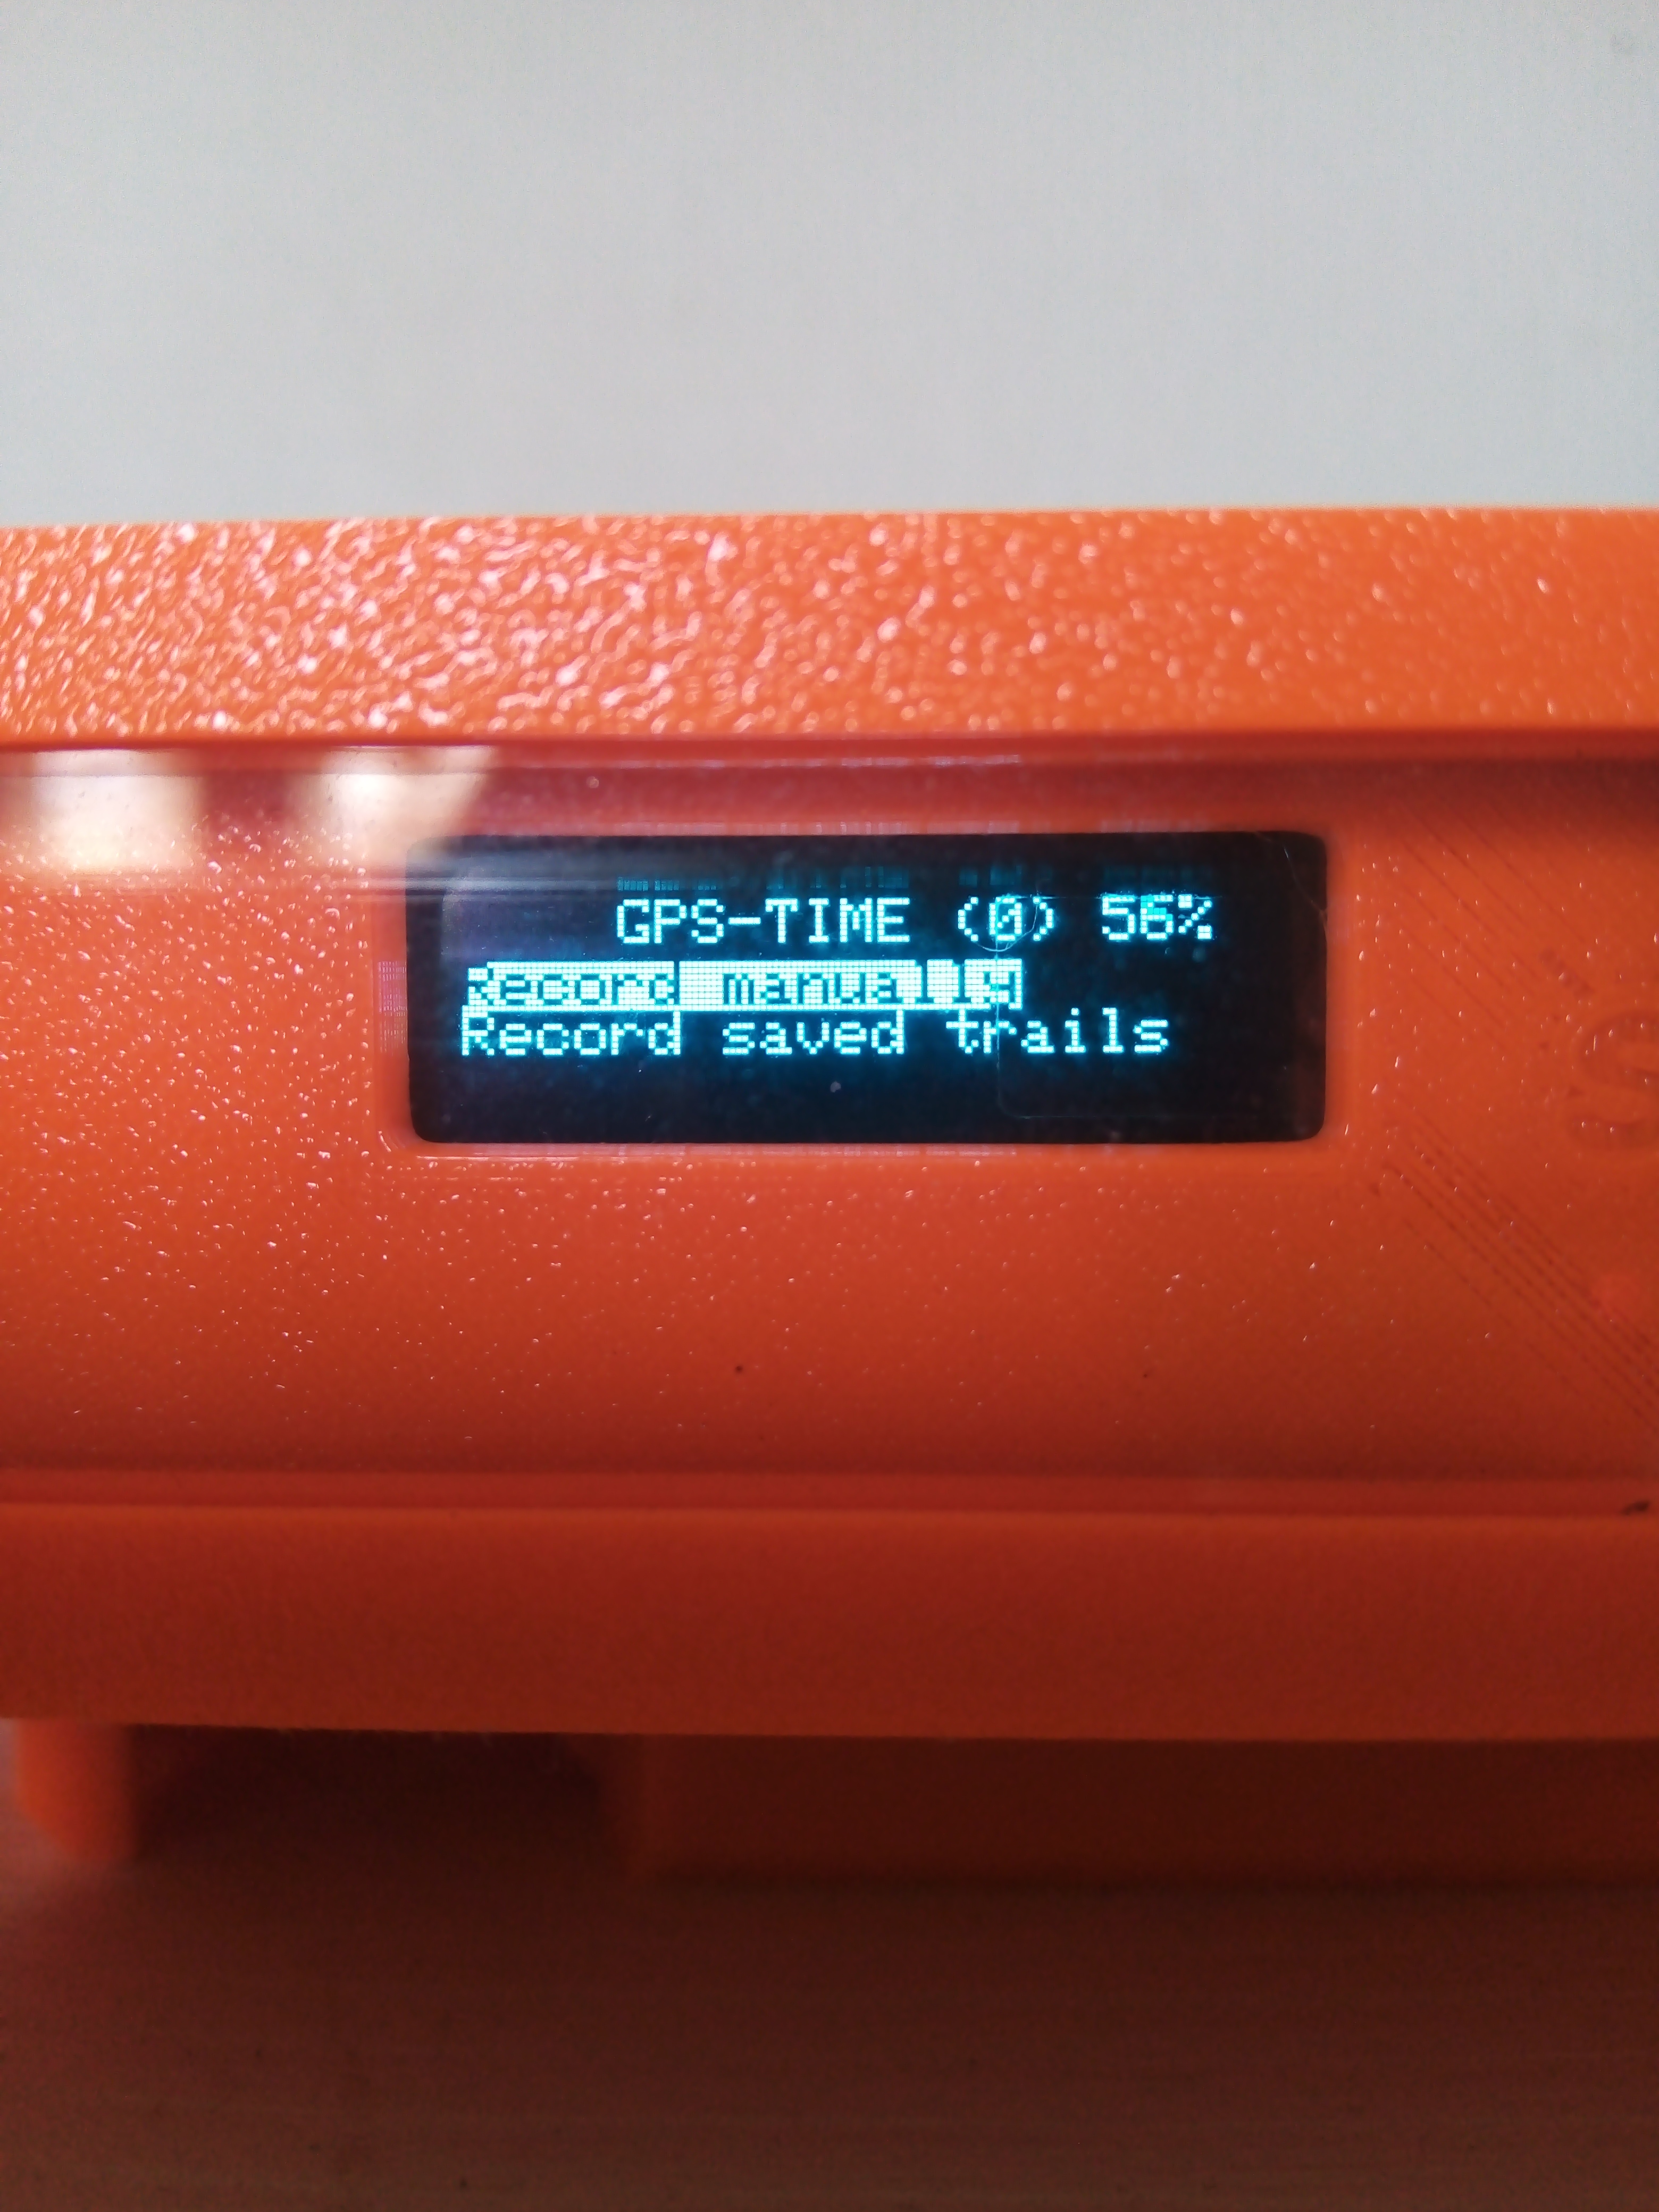
\includegraphics[width=65mm]{Figures/screen_view.jpg}
    \caption{The main menu layout.}
    \label{fig:menu_screen}
\end{figure}



\subsection{Specs of the device as a table}


\begin{longtable}{ |p{0.3\linewidth} | p{0.5\linewidth}|} 
    \caption{The important specifications of the device.}
    \label{tab:specs}\\
     \hline
     Property & Value \\ 
     \hline
     \hline
     Measured variables & Front damper position, rear damper position, frame acceleration, braking, location, speed, elevation, elapsed time\\
     \hline
     Additional features & Sag measuring, quick data review with BLE*, automatic rear sensor detection, gpx track segment based recording, *Proper phone app still missing, but values can be read \\
     \hline
     \newpage
     \hline
     Linear sensor range & 0-300 mm\\
     \hline
     Linear sensor resolution & 0.07 mm\\
     \hline
     Accelerometer range & $\pm$20g\\
     \hline
     Sample rate & Adjustable: max 180 Hz (350 Hz GPS off)\\
     \hline
     Max SD card size & 32 GB (microSD card, type SD or SDHC, not compatible with SDXC or higher)\\
     \hline
     Battery life & approx. 8 h measuring\\
     \hline
     Waterproof & Splash waterproof\\
     \hline
     Powering options & Internal battery or external 7-12 V DC\\
     \hline
     Number cable ties needed for installation & 10 - 15, depending on the number of integrated threads on the frame\\
     \hline
     Main unit dimensions & 180x68x28 mm\\
     \hline
     Weight & 285 g main unit + 210 g sensors\\
     \hline
     Final budget & $\approx$ 200€\\     
     \hline
\end{longtable}
    

\subsection{Conclusions}

Did the project meet its requirements? Mainly yes, as the first three requirements of the project plan section are fulfilled and the latter two work to some point. The device ended up having more features than originally planned and the data review without PC didn't get enough attention. There is one fundamental problem in the design of the data review functionality, which reduces the usefulness of it: The BLE communication is designed for small amounts of data, so the idea of sending complete files to smartphone for plotting was realized to not work. The current data review with averages and maximum values gives some feedback, but if the trail has different sections, the user can't get any specific feedback from the different sections. From this point of view the data review should be done with WiFi and it could even be done so that the microcontroller runs a web server that has its own plotting code and the user just visits the page to review the data. This would of course need different main board, for instance an ESP32 or Raspberry pi zero.

The bonus requirement about the cost is a bit tricky, as the final budget of 200 euros isn't cheap, but it's still around 10\% of the cost of a commercial solution. One could probably save up to 40 euros by finding the cheapest retailers and of course it is possible to simplify the device, for instance by leaving out the GPS, and save money that way. The alternative component choices in section 5.1 considers some other components, that are either cheaper or better. On the other end, one could argue that the project is quite cheap, when looking at the price of one weatherproof linear potentiometer that could be used in this project, as it costs 330 euros (versus the used DIY string pot cost under 20 euros).

Apart from the data review the project turned out to be working quite well and it definitely proofs that one can build a proper mountain bike suspension setup tool with basic electronics stuff. The external sensors work well and the main unit is compact enough to fit on to a bike without disturbing the rider. One small thing that is probably updated soon is that now the potentiometers are supported only by their bushings, so adding a bearing to the linear sensor would probably increase the life of the potentiometer. This update requires only a new reel for the string as the enclosure is designed to fit a 61901 bearing. Other design issue is that the ceramic patch antenna of the used GPS module is not especially fast when it comes to finding fix in urban areas, so it would have been good to choose a module with external antenna option. Of course there are a lot of small things that could be improved, for instance the efficiency of the program code and the powering solution. Now there is 5 V boost-converter and 3.3 V regulator between the board and the battery, but changing these to one 3.3 V buck/boost-converter would improve the power efficiency. These things are connected though, as the Nano can't take 3.3 V input unless you cut the solder pad of the regulator, but cutting the pad means that no new program code can be uploaded to the Nano. So this powering optimization would need a small switch on board that toggles between program mode and direct current mode.

The device has many features that offer easy upgrades in the future. One of these is the fact, that the rear sensor has two analog signal channels, one of which is now used for detecting the rear sensor. This means that it is possible to make a rear sensor that has two elongation strips and would allow one to study the behavior of different frame materials on a hardtail bike, by attaching the elongation strips to seatstay tubes of the rear triangle. This would give some quantitative results to the never ending debate whether steel and titanium offer a softer frame characteristics than aluminium. Another future upgrade would be to use all the data that the IMU offers, not just the acceleration, and combine it with GPS to make sensor fusion positioning. These upgrades are easily doable as there is still over half of the program memory left on the Nano, although the current code is already nearly 2000 lines long and uses 10 libraries.


\newpage
\section{How to build the project and alternative part lists}
\rule{12.7cm}{0.4pt}

\subsection{Alternative component choices}

The components of the project from a quite well working package and it's worth noting that the used code only works on mbed architecture boards. Another fact is that the code currently takes about 0.4 MB of program memory, so going with smaller/cheaper microcontroller means that some features will need to be discarded. When looking for GPS module, one should choose a model that has a possibility to mount an external antenna, as it will make getting the GPS fix way faster. A small side note here: The Nano 33 BLE is actually the most powerful Arduino board in terms of clock speed and memory (64 MHz and 1 MB/256 kB), if we don't count the Portenta, which is designed for the industry. These in mind there are three alternative component lists below:

\begin{itemize}
    \item Willing to reach faster sample rates?
    \begin{itemize}
        \item For microcontroller unit choose a Teensy 4.0 or higher, these boards run at 600 MHz, have even more memory, are Adruino IDE compatible and cheaper than the Nano. The Teensy 4.1 even has on board microSD slot. Teensys also have emulated EEPROM, which means that one can save settings easily. 
        \item For GPS module choose a Sparkfun module with antenna connection.
        \item As the Teensy doesn't have IMU or BLE, you should get those separately and probably go with some other wireless connection.
    \end{itemize} 

    \item Looking for more budget friendly option?
    \begin{itemize}
        \item Leaving out the GPS will save money and in case you don't need wireless connection you can save even more.
        \item For microcontroller unit choosing Adafruits Feather M0 adalogger will combine the microSD adapter to the same board. Keep in mind that this and other samd architecture boards run at 48 MHz and have only as much program memory 256kB as the Nano has RAM, so there can't be as much features with these boards.
    \end{itemize}

    \item Bare minimum?
    \begin{itemize}
        \item Microcontroller unit: Seeeduino XIAO - costs 8,80 € in Partco or Raspberry Pi Pico - 8,80€.
        \item Use only external sensors, 3-axis I2C accelerometer, microSD adapter and the OLED display.
        \item With these the cost will be about 120 €, when purchasing components from Finnish shops.
    \end{itemize}
    
\end{itemize}


\subsection{Light building instructions}

The building process is quite simple if one has access to a 3D printer and soldering tools. If going with the same components, the component layout pictured in section 3.1 should work. In case using different components, one should first cut a 145x55 mm piece of pcb (or draw rectangle on paper and place the components on that) and test fit all the components. After making sure that the components fit, the parts need to be 3D printed according to notes described in section 5.3, note that the pause prints need some components to prepared, for instance the brake switches with wires soldered on place and the 3 mm plexigass cut to correct dimensions 147x23 mm.

After all the parts are printed the potentiometers can be assembled by first inserting the spring to the bottom part of the cover and attaching the string to the reel and the ball at the end of the string. It is also good to make sure that the tolerance between the potentiometer shaft and the reel is sufficient. In case it is too tight, one can try to use a 6.3 mm drill bit to take off some material. When everything fits together, install the reel to the spring (with the string nearly entirely wound on to the reel) and add a bit of preload to the spring and push the potentiometer in. After this tighten the potentiometer nut and solder some 3-pole wire with enough length (max diameter 6 mm) to the potentiometer. Plus goes to 1, GND goes to 3 and signal goes to solder pad no. 2 (numbers are valid for the potentiometer pictured in section 3.1). After this, route the wire through the top cover and screw the cover in place with 2x 20 mm M3 screws. Repeat same procedure for the other potentiometer.

To finish the external sensors, take some 5-pole wire and measure it so that it reaches from the handlebar to the water bottle mount. Then solder the brake sensors and the front potentiometer to the 5-pole wire according to the schematic found at the bottom of this section. Insulate the connections with hot glue and shrinking tube. The 3-pole wire of the rear sensor is attached directly to the rear sensor connector according to the schematic, but in addition you must connect the pin 4 of the connector to GND, in order for the automatic rear sensor detection to work.

The main electronics should be connected with quite small wire to save space underneath the pcb (see figure on section 3.1). After decorating the pcb according to the schematic, one should install the connectors and buttons to the main enclosure, screw the battery on its place (3x 10 mm M3). Then solder the connector and button wires to the pcb. After this carefully press the pcb in to the slot in the enclosure and use a 10 mm M3 screw to secure it to its place. Now just upload the code to the board (it takes some 15 minutes to compile and upload) and test the device. If everything works, screw the enclosure lid (4x 20 mm M3) and front plate (2x 7 mm M3 countersunk) on their places, if not check the connections. After this mount the enclosure door with 25 mm M3 screw and attach your preferred mounting solution to the bottom of the enclosure with 10 mm M3 screws. Now the device is ready, just plug in a memory card and start data logging.

Figure \ref{fig:schematic} below shows the schematic of the device, note that the pins of the Nano 33 BLE are numbered according to their place not according to A0, A1, ..., D2, Rx.., the USB port is at the opposite end to the IC notch, e.g. between pins 15 and 16.

\begin{figure}[H]
    \centering
    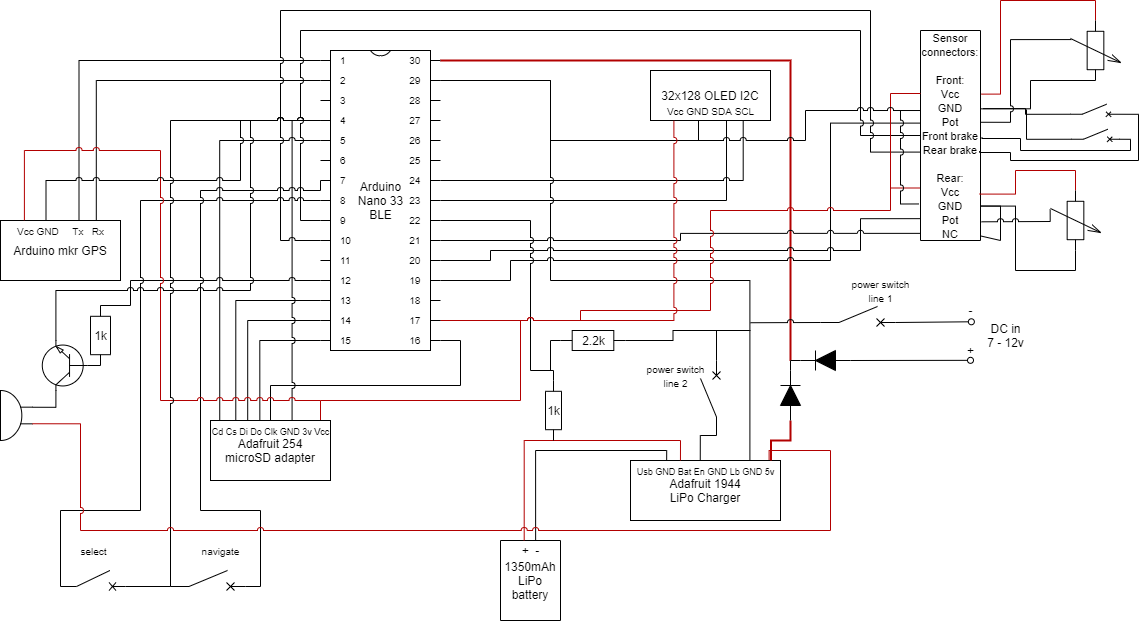
\includegraphics[width=105mm]{Figures/schematic.png}
    \caption{The wiring schematic for all the components. Made using \texttt{draw.io}.}
    \label{fig:schematic}
\end{figure}

Note that the schematic in figure \ref{fig:schematic} applies perfectly only for the components mentioned in the components list in section 2. Especially the GPS serial wiring is opposite to standard serial, as the used module is designed to be used as a shield rather than a separate module. So in case you are using 'normal' GPS module the serial wiring should be gps(tx) → 2 (nano rx1) and gps(rx) → 1 (nano tx1).


\subsection{3D printing specifications}

All the parts were printed with PrusaSlicer default settings for Prusa Mini in PETG 0.2 mm speed mode: Nozzle temperature 250°c, heat bed temperature 90°c, 0.2 mm layer height, 20\% infill, rectangular infill pattern, skirt on, no brim and when using supports the detect bridging perimeters option was set on. Used nozzle was standard 0.4 mm one and the used spring steel sheet (removable build plate) was the textured one, which is recommended for PETG. Pause prints were made during slicing to prevent forgetting them. For the smaller and more detailed parts, for instance the front plate, a smaller 0.15 mm layer height might also be used. The amount of supports used is quite minimal and depending of the capabilities of the used printer the models might need more supports than mentioned in table \ref{tab:printing}. Table \ref{tab:printing} shows also some slicing notes for the 3D models.


\begin{longtable}{ |p{0.35\linewidth} | p{0.3\linewidth}| p{0.25\linewidth}| p{0.15\linewidth}|} 
    \caption{Notes for 3D printing the parts for the project.}
    \label{tab:printing}\\
     \hline
     Model & Orientation & Pause prints & Supports \\ 
     \hline
     \hline
     brake\_sensor & horizontal & 1, the micro switch and its wires & - \\
     \hline
     enclosure\_50mm\_ round\_adapter &	bolt holes horizontally &	0 &	-\\
     \hline
     enclosure\_battery\_holder &	largest flat face to build plate &	0 &	-\\
     \hline
     enclosure\_dc\_in\_cap &	textured side to build plate &	0 &	-\\
     \hline
     enclosure\_door &	non-grooved face to build plate &	1, insert the plexiglass (147x23x3 mm) &	support enforcer for the knob cutout\\
     \hline
     enclosure\_fidlock\_adapter	& largest flat face to build plate &	1, insert M6 washers (1.5mm thick) to the cutouts &	-\\
     \hline
     enclosure\_front\_plate &	textured side to build plate &	0 &	-\\
     \hline
     enclosure\_lid &	hole side up &	1, 4 x M3 hex nuts &	-\\
     \hline
     enclosure\_m4\_knob &	cut to half and the uncut flat faces to build plate &	0 &	the other half with hole needs supports from build plate\\
     \hline
     enclosure\_main\_part &	horizontal &	5, insert M3 nuts (3 x square, 8 x hex) &	- \\
     \hline
     \newpage
     \hline
     enclosure\_sensor\_cap &	text side to build plate &	0 &	-\\
     \hline
     enclosure\_triangle\_ adapter &	bolt holes horizontally &	0 &	-\\
     \hline
     enclosure\_usb\_lid &	textured side to build plate &	0 &	-\\
     \hline
     pcb\_254\_nut &	holes vertically &	0 &	-\\
     \hline
     pcb\_254\_spacer &	holes vertically &	0 &	-\\
     \hline
     pcb\_1944\_nut &	holes vertically &	0 &	-\\
     \hline
     pcb\_1944\_spacer &	holes vertically &	0 &	-\\
     \hline
     pcb\_screen\_holder &	holes horizontally &	0 &	-\\
     \hline
     pot\_adapter\_m5 &	horizontal &	0 &	supports from build plate\\
     \hline
     pot\_ball\_holder\_fork &	flat face to the build plate & 0 &	-\\
     \hline
     pot\_ball\_holder\_shock &	flat face to the build plate &	0 &	-\\
     \hline
     pot\_ball\_joint &	flat face to the build plate &	0 &	-\\
     \hline
     pot\_cover\_bottom &	potentiometer hole vertically, with the cut edges of the cylinder at the same level &	1, insert 2 x square M3 nuts &	-\\
     \hline
     pot\_cover\_top &	the round flat end to the build plate &	0 &	-\\
     \hline
     pot\_fork\_adapter &	vertically, flat half circle to the build plate &	0 &	supports from build plate\\
     \hline
     pot\_reel	& the potentiometer axle hole to the build plate &	0 &	-\\
     \hline
     pot\_wheel &	flat face to the build plate &	0 &	-\\
     \hline
      pot\_wheel\_arm &	flat face to the build plate &	1, insert hex M3 nut & -\\
     \hline
\end{longtable}



\end{document}

\begin{figure}[H]
    \centering
    \includegraphics[width=105mm]{exercise1_model.PNG}
    \caption{Simulation model for the acceleration.}
    \label{kuva1}
\end{figure}

\begin{align}
    \frac{d}{dt} x(t) &= ax(t) - bx(t)y(t)\label{yht3}\\
    \frac{d}{dt} y(t) &= -py(t) + qx(t)y(t)\label{yht4}
\end{align}
